%!TEX spellcheck
%!TEX jobname = ti3allinone
%!TEX output_directory = out
%%%%%%%%%%%%%%%%%%%%%%%%%%%%%%%%%%%%%%%%%
%  My documentation report
%  Objetive: Explain what I did and how, so someone can continue with the investigation
%
% Important note:
% Chapter heading images should have a 2:1 width:height ratio,
% e.g. 920px width and 460px height.
%
%%%%%%%%%%%%%%%%%%%%%%%%%%%%%%%%%%%%%%%%%

%----------------------------------------------------------------------------------------
%	PACKAGES AND OTHER DOCUMENT CONFIGURATIONS
%----------------------------------------------------------------------------------------

\documentclass[11pt,fleqn]{book} % Default font size and left-justified equations

\usepackage[top=3cm,bottom=3cm,left=3.2cm,right=3.2cm,headsep=10pt,letterpaper]{geometry} % Page margins

\usepackage{xcolor} % Required for specifying colors by name
\definecolor{ocre}{RGB}{80,130,201} % Define the orange color used for highlighting throughout the book

% Font Settings
\usepackage{avant} % Use the Avantgarde font for headings
%\usepackage{times} % Use the Times font for headings
\usepackage{mathptmx} % Use the Adobe Times Roman as the default text font together with math symbols from the Sym­bol, Chancery and Com­puter Modern fonts

\usepackage{microtype} % Slightly tweak font spacing for aesthetics
\usepackage[utf8]{inputenc} % Required for including letters with accents
\usepackage[T1]{fontenc} % Use 8-bit encoding that has 256 glyphs

% Bibliography
\usepackage[style=alphabetic,sorting=nyt,sortcites=true,autopunct=true,babel=hyphen,hyperref=true,abbreviate=false,backref=true,backend=biber]{biblatex}
\addbibresource{bibliography.bib} % BibTeX bibliography file
\defbibheading{bibempty}{}

%----------------------------------------------------------------------------------------
%	VARIOUS REQUIRED PACKAGES
%----------------------------------------------------------------------------------------

\usepackage{titlesec} % Allows customization of titles

\usepackage{graphicx} % Required for including pictures
\graphicspath{{Pictures/}} % Specifies the directory where pictures are stored

\usepackage{lipsum} % Inserts dummy text

\usepackage{tikz} % Required for drawing custom shapes

\usepackage[english]{babel} % English language/hyphenation

\usepackage{enumitem} % Customize lists
\setlist{nolistsep} % Reduce spacing between bullet points and numbered lists

\usepackage{booktabs} % Required for nicer horizontal rules in tables

\usepackage{eso-pic} % Required for specifying an image background in the title page

\usepackage{float}

%----------------------------------------------------------------------------------------
%	MAIN TABLE OF CONTENTS
%----------------------------------------------------------------------------------------

\usepackage{titletoc} % Required for manipulating the table of contents

\contentsmargin{0cm} % Removes the default margin
% Chapter text styling
\titlecontents{chapter}[1.25cm] % Indentation
{\addvspace{15pt}\large\sffamily\bfseries} % Spacing and font options for chapters
{\color{ocre!60}\contentslabel[\Large\thecontentslabel]{1.25cm}\color{ocre}} % Chapter number
{}  
{\color{ocre!60}\normalsize\sffamily\bfseries\;\titlerule*[.5pc]{.}\;\thecontentspage} % Page number
% Section text styling
\titlecontents{section}[1.25cm] % Indentation
{\addvspace{5pt}\sffamily\bfseries} % Spacing and font options for sections
{\contentslabel[\thecontentslabel]{1.25cm}} % Section number
{}
{\sffamily\hfill\color{black}\thecontentspage} % Page number
[]
% Subsection text styling
\titlecontents{subsection}[1.25cm] % Indentation
{\addvspace{1pt}\sffamily\small} % Spacing and font options for subsections
{\contentslabel[\thecontentslabel]{1.25cm}} % Subsection number
{}
{\sffamily\;\titlerule*[.5pc]{.}\;\thecontentspage} % Page number
[] 

%----------------------------------------------------------------------------------------
%	MINI TABLE OF CONTENTS IN CHAPTER HEADS
%----------------------------------------------------------------------------------------

% Section text styling
\titlecontents{lsection}[0em] % Indendating
{\footnotesize\sffamily} % Font settings
{}
{}
{}

% Subsection text styling
\titlecontents{lsubsection}[.5em] % Indentation
{\normalfont\footnotesize\sffamily} % Font settings
{}
{}
{}
 
%----------------------------------------------------------------------------------------
%	PAGE HEADERS
%----------------------------------------------------------------------------------------

\usepackage{fancyhdr} % Required for header and footer configuration

\pagestyle{fancy}
\renewcommand{\chaptermark}[1]{\markboth{\sffamily\normalsize\bfseries\chaptername\ \thechapter.\ #1}{}} % Chapter text font settings
\renewcommand{\sectionmark}[1]{\markright{\sffamily\normalsize\thesection\hspace{5pt}#1}{}} % Section text font settings
\fancyhf{} \fancyhead[LE,RO]{\sffamily\normalsize\thepage} % Font setting for the page number in the header
\fancyhead[LO]{\rightmark} % Print the nearest section name on the left side of odd pages
\fancyhead[RE]{\leftmark} % Print the current chapter name on the right side of even pages
\renewcommand{\headrulewidth}{0.5pt} % Width of the rule under the header
\addtolength{\headheight}{2.5pt} % Increase the spacing around the header slightly
\renewcommand{\footrulewidth}{0pt} % Removes the rule in the footer
\fancypagestyle{plain}{\fancyhead{}\renewcommand{\headrulewidth}{0pt}} % Style for when a plain pagestyle is specified

% Removes the header from odd empty pages at the end of chapters
\makeatletter
\renewcommand{\cleardoublepage}{
\clearpage\ifodd\c@page\else
\hbox{}
\vspace*{\fill}
\thispagestyle{empty}
\newpage
\fi}

%----------------------------------------------------------------------------------------
%	THEOREM STYLES
%----------------------------------------------------------------------------------------

\usepackage{amsmath,amsfonts,amssymb,amsthm} % For math equations, theorems, symbols, etc

\newcommand{\intoo}[2]{\mathopen{]}#1\,;#2\mathclose{[}}
\newcommand{\ud}{\mathop{\mathrm{{}d}}\mathopen{}}
\newcommand{\intff}[2]{\mathopen{[}#1\,;#2\mathclose{]}}
\newtheorem{notation}{Notation}[chapter]

%%%%%%%%%%%%%%%%%%%%%%%%%%%%%%%%%%%%%%%%%%%%%%%%%%%%%%%%%%%%%%%%%%%%%%%%%%%
%%%%%%%%%%%%%%%%%%%% dedicated to boxed/framed environements %%%%%%%%%%%%%%
%%%%%%%%%%%%%%%%%%%%%%%%%%%%%%%%%%%%%%%%%%%%%%%%%%%%%%%%%%%%%%%%%%%%%%%%%%%
\newtheoremstyle{ocrenumbox}% % Theorem style name
{0pt}% Space above
{0pt}% Space below
{\normalfont}% % Body font
{}% Indent amount
{\small\bf\sffamily\color{ocre}}% % Theorem head font
{\;}% Punctuation after theorem head
{0.25em}% Space after theorem head
{\small\sffamily\color{ocre}\thmname{#1}\nobreakspace\thmnumber{\@ifnotempty{#1}{}\@upn{#2}}% Theorem text (e.g. Theorem 2.1)
\thmnote{\nobreakspace\the\thm@notefont\sffamily\bfseries\color{black}---\nobreakspace#3.}} % Optional theorem note
\renewcommand{\qedsymbol}{$\blacksquare$}% Optional qed square

\newtheoremstyle{blacknumex}% Theorem style name
{5pt}% Space above
{5pt}% Space below
{\normalfont}% Body font
{} % Indent amount
{\small\bf\sffamily}% Theorem head font
{\;}% Punctuation after theorem head
{0.25em}% Space after theorem head
{\small\sffamily{\tiny\ensuremath{\blacksquare}}\nobreakspace\thmname{#1}\nobreakspace\thmnumber{\@ifnotempty{#1}{}\@upn{#2}}% Theorem text (e.g. Theorem 2.1)
\thmnote{\nobreakspace\the\thm@notefont\sffamily\bfseries---\nobreakspace#3.}}% Optional theorem note

\newtheoremstyle{blacknumbox} % Theorem style name
{0pt}% Space above
{0pt}% Space below
{\normalfont}% Body font
{}% Indent amount
{\small\bf\sffamily}% Theorem head font
{\;}% Punctuation after theorem head
{0.25em}% Space after theorem head
{\small\sffamily\thmname{#1}\nobreakspace\thmnumber{\@ifnotempty{#1}{}\@upn{#2}}% Theorem text (e.g. Theorem 2.1)
\thmnote{\nobreakspace\the\thm@notefont\sffamily\bfseries---\nobreakspace#3.}}% Optional theorem note

%%%%%%%%%%%%%%%%%%%%%%%%%%%%%%%%%%%%%%%%%%%%%%%%%%%%%%%%%%%%%%%%%%%%%%%%%%%
%%%%%%%%%%%%% dedicated to non-boxed/non-framed environements %%%%%%%%%%%%%
%%%%%%%%%%%%%%%%%%%%%%%%%%%%%%%%%%%%%%%%%%%%%%%%%%%%%%%%%%%%%%%%%%%%%%%%%%%
\newtheoremstyle{ocrenum}% % Theorem style name
{5pt}% Space above
{5pt}% Space below
{\normalfont}% % Body font
{}% Indent amount
{\small\bf\sffamily\color{ocre}}% % Theorem head font
{\;}% Punctuation after theorem head
{0.25em}% Space after theorem head
{\small\sffamily\color{ocre}\thmname{#1}\nobreakspace\thmnumber{\@ifnotempty{#1}{}\@upn{#2}}% Theorem text (e.g. Theorem 2.1)
\thmnote{\nobreakspace\the\thm@notefont\sffamily\bfseries\color{black}---\nobreakspace#3.}} % Optional theorem note
\renewcommand{\qedsymbol}{$\blacksquare$}% Optional qed square
\makeatother

% Defines the theorem text style for each type of theorem to one of the three styles above
\newcounter{dummy} 
\numberwithin{dummy}{section}
\theoremstyle{ocrenumbox}
\newtheorem{theoremeT}[dummy]{Theorem}
\newtheorem{problem}{Problem}[chapter]
\newtheorem{exerciseT}{Exercise}[chapter]
\theoremstyle{blacknumex}
\newtheorem{exampleT}{Example}[chapter]
\theoremstyle{blacknumbox}
\newtheorem{vocabulary}{Vocabulary}[chapter]
\newtheorem{definitionT}{Definition}[section]
\newtheorem{corollaryT}[dummy]{Corollary}
\theoremstyle{ocrenum}
\newtheorem{proposition}[dummy]{Proposition}

%----------------------------------------------------------------------------------------
%	
%----------------------------------------------------------------------------------------

\RequirePackage[framemethod=default]{mdframed} % Required for creating the theorem, definition, exercise and corollary boxes

\newmdenv[skipabove=7pt,
skipbelow=7pt,
rightline=false,
leftline=true,
topline=false,
bottomline=false,
backgroundcolor=blue!8,
linecolor=blue!80,
innerleftmargin=5pt,
innerrightmargin=5pt,
innertopmargin=5pt,
innerbottommargin=5pt,
leftmargin=0cm,
rightmargin=0cm,
linewidth=4pt]{SEbox}  
\newenvironment{SEf}{\textcolor{blue}}


% Shards of the Throne Expansion box	  
% \newmdenv[skipabove=7pt,
% skipbelow=7pt,
% rightline=false,
% leftline=true,
% topline=false,
% bottomline=false,
% backgroundcolor=red!6,
% linecolor=red!70,
% innerleftmargin=5pt,
% innerrightmargin=5pt,
% innertopmargin=5pt,
% innerbottommargin=5pt,
% leftmargin=0cm,
% rightmargin=0cm,
% linewidth=4pt]{STbox}	
\newmdenv[leftmargin=0cm,backgroundcolor=red]{STbox}    
\newenvironment{STf}{\textcolor{red}}

% Online Rules and Options from the FFG-Website box
\newmdenv[skipabove=7pt,
skipbelow=7pt,
rightline=false,
leftline=true,
topline=false,
bottomline=false,
linecolor=green,
backgroundcolor=green!15,
innerleftmargin=5pt,
innerrightmargin=5pt,
innertopmargin=0pt,
leftmargin=0cm,
rightmargin=0cm,
linewidth=4pt,
innerbottommargin=0pt]{FFGbox}	
\newenvironment{FFGf}{\color[rgb]{0.1,0.5,0.1}}

% Corollary box
\newmdenv[skipabove=7pt,
skipbelow=7pt,
rightline=false,
leftline=true,
topline=false,
bottomline=false,
linecolor=black!50,
backgroundcolor=black!5,
innerleftmargin=5pt,
innerrightmargin=5pt,
innertopmargin=5pt,
leftmargin=0cm,
rightmargin=0cm,
linewidth=4pt,
innerbottommargin=5pt]{HRbox}
\newenvironment{HRf}{\textcolor{black!50}}

% Creates an environment for each type of theorem and assigns it a theorem text style from the "Theorem Styles" section above and a colored box from above


%----------------------------------------------------------------------------------------
%	SUBSECTIONS ENVIRONMENTS
%----------------------------------------------------------------------------------------

\newenvironment{remark}{\par\vspace{10pt}\small % Vertical white space above the remark and smaller font size
\begin{list}{}{
\leftmargin=35pt % Indentation on the left
\rightmargin=25pt}\item\ignorespaces % Indentation on the right
\makebox[-2.5pt]{\begin{tikzpicture}[overlay]
\node[draw=ocre!60,line width=1pt,circle,fill=ocre!25,font=\sffamily\bfseries,inner sep=1pt,outer sep=0pt] at (-18pt,0pt){\textcolor{ocre}{remark}};\end{tikzpicture}} % Orange symbol in a circle
\advance\baselineskip -1pt}{\end{list}\vskip5pt} % Tighter line spacing and white space after remark


% \newenvironment{SE}{\par\vspace{10pt}\small % Vertical white space above the remark and smaller font size
% \begin{list}{}{
% \leftmargin=35pt % Indentation on the left
% \rightmargin=25pt}\item\ignorespaces % Indentation on the right
% \makebox[-2.5pt]{\begin{tikzpicture}[overlay]
% \node[draw=ocre!60,line width=1pt,circle,fill=ocre!25,font=\sffamily\bfseries,inner sep=1pt,outer sep=0pt] at (-18pt,0pt){\textcolor{ocre}{SE}};\end{tikzpicture}} % Orange symbol in a circle
% \advance\baselineskip -1pt}{\end{list}\vskip5pt} % Tighter line spacing and white space after remark


% \newenvironment{SoT}{\par\vspace{10pt}\small % Vertical white space above the remark and smaller font size
% \begin{list}{}{
% \leftmargin=35pt % Indentation on the left
% \rightmargin=25pt}\item\ignorespaces % Indentation on the right
% \makebox[-2.5pt]{\begin{tikzpicture}[overlay]
% \node[draw=ocre!60,line width=1pt,circle,fill=ocre!25,font=\sffamily\bfseries,inner sep=1pt,outer sep=0pt] at (-18pt,0pt){\textcolor{ocre}{SoT}};\end{tikzpicture}} % Orange symbol in a circle
% \advance\baselineskip -1pt}{\end{list}\vskip5pt} % Tighter line spacing and white space after remark


% \newenvironment{FFG}{\par\vspace{10pt}\small % Vertical white space above the remark and smaller font size
% \begin{list}{}{
% \leftmargin=35pt % Indentation on the left
% \rightmargin=25pt}\item\ignorespaces % Indentation on the right
% \makebox[-2.5pt]{\begin{tikzpicture}[overlay]
% \node[draw=ocre!60,line width=1pt,circle,fill=ocre!25,font=\sffamily\bfseries,inner sep=1pt,outer sep=0pt] at (-18pt,0pt){\textcolor{ocre}{FFG}};\end{tikzpicture}} % Orange symbol in a circle
% \advance\baselineskip -1pt}{\end{list}\vskip5pt} % Tighter line spacing and white space after remark


% \newenvironment{HR}{\par\vspace{10pt}\small % Vertical white space above the remark and smaller font size
% \begin{list}{}{
% \leftmargin=35pt % Indentation on the left
% \rightmargin=25pt}\item\ignorespaces % Indentation on the right
% \makebox[-2.5pt]{\begin{tikzpicture}[overlay]
% \node[draw=ocre!60,line width=1pt,circle,fill=ocre!25,font=\sffamily\bfseries,inner sep=1pt,outer sep=0pt] at (-18pt,0pt){\textcolor{ocre}{HR}};\end{tikzpicture}} % Orange symbol in a circle
% \advance\baselineskip -1pt}{\end{list}\vskip5pt} % Tighter line spacing and white space after remark


%   SUBSECTIONS ENVIRONMENTS

\usepackage{framed}
%----------------------------------------------------------------------------------------
%	SECTION NUMBERING IN THE MARGIN
%----------------------------------------------------------------------------------------

\makeatletter
\renewcommand{\@seccntformat}[1]{\llap{\textcolor{ocre}{\csname the#1\endcsname}\hspace{1em}}}                    
\renewcommand{\section}{\@startsection{section}{1}{\z@}
{-4ex \@plus -1ex \@minus -.4ex}
{1ex \@plus.2ex }
{\normalfont\large\sffamily\bfseries}}
\renewcommand{\subsection}{\@startsection {subsection}{2}{\z@}
{-3ex \@plus -0.1ex \@minus -.4ex}
{0.5ex \@plus.2ex }
{\normalfont\sffamily\bfseries}}
\renewcommand{\subsubsection}{\@startsection {subsubsection}{3}{\z@}
{-2ex \@plus -0.1ex \@minus -.2ex}
{.2ex \@plus.2ex }
{\normalfont\small\sffamily\bfseries}}                        
\renewcommand\paragraph{\@startsection{paragraph}{4}{\z@}
{-2ex \@plus-.2ex \@minus .2ex}
{.1ex}
{\normalfont\small\sffamily\bfseries}}


%----------------------------------------------------------------------------------------
%	HYPERLINKS IN THE DOCUMENTS
%----------------------------------------------------------------------------------------

% For an unclear reason, the package should be loaded now and not later
\usepackage{hyperref}
\hypersetup{hidelinks,backref=true,pagebackref=true,hyperindex=true,colorlinks=false,breaklinks=true,urlcolor= ocre,bookmarks=true,bookmarksopen=false,pdftitle={Title},pdfauthor={Author}}

%----------------------------------------------------------------------------------------
%	CHAPTER HEADINGS
%----------------------------------------------------------------------------------------

% The set-up below should be (sadly) manually adapted to the overall margin page septup controlled by the geometry package loaded in the main.tex document. It is possible to implement below the dimensions used in the goemetry package (top,bottom,left,right)... TO BE DONE

\newcommand{\thechapterimage}{}
\newcommand{\chapterimage}[1]{\renewcommand{\thechapterimage}{#1}}

% Numbered chapters with mini tableofcontents
\def\thechapter{\arabic{chapter}}
\def\@makechapterhead#1{
\thispagestyle{empty}
{\centering \normalfont\sffamily
\ifnum \c@secnumdepth >\m@ne
\if@mainmatter
\startcontents
\begin{tikzpicture}[remember picture,overlay]
\node at (current page.north west)
{\begin{tikzpicture}[remember picture,overlay]
\node[anchor=north west,inner sep=0pt] at (0,0) {\includegraphics[width=\paperwidth]{\thechapterimage}};
%%%%%%%%%%%%%%%%%%%%%%%%%%%%%%%%%%%%%%%%%%%%%%%%%%%%%%%%%%%%%%%%%%%%%%%%%%%%%%%%%%%%%
% Commenting the 3 lines below removes the small contents box in the chapter heading
%\fill[color=ocre!10!white,opacity=.6] (1cm,0) rectangle (8cm,-7cm);
%\node[anchor=north west] at (1.1cm,.35cm) {\parbox[t][8cm][t]{6.5cm}{\huge\bfseries\flushleft \printcontents{l}{1}{\setcounter{tocdepth}{2}}}};
\draw[anchor=west] (5cm,-9cm) node [rounded corners=20pt,fill=ocre!10!white,text opacity=1,draw=ocre,draw opacity=1,line width=1.5pt,fill opacity=.6,inner sep=12pt]{\huge\sffamily\bfseries\textcolor{black}{\thechapter. #1\strut\makebox[22cm]{}}};
%%%%%%%%%%%%%%%%%%%%%%%%%%%%%%%%%%%%%%%%%%%%%%%%%%%%%%%%%%%%%%%%%%%%%%%%%%%%%%%%%%%%%
\end{tikzpicture}};
\end{tikzpicture}}
\par\vspace*{230\p@}
\fi
\fi}

% Unnumbered chapters without mini tableofcontents (could be added though) 
\def\@makeschapterhead#1{
\thispagestyle{empty}
{\centering \normalfont\sffamily
\ifnum \c@secnumdepth >\m@ne
\if@mainmatter
\begin{tikzpicture}[remember picture,overlay]
\node at (current page.north west)
{\begin{tikzpicture}[remember picture,overlay]
\node[anchor=north west,inner sep=0pt] at (0,0) {\includegraphics[width=\paperwidth]{\thechapterimage}};
\draw[anchor=west] (5cm,-9cm) node [rounded corners=20pt,fill=ocre!10!white,fill opacity=.6,inner sep=12pt,text opacity=1,draw=ocre,draw opacity=1,line width=1.5pt]{\huge\sffamily\bfseries\textcolor{black}{#1\strut\makebox[22cm]{}}};
\end{tikzpicture}};
\end{tikzpicture}}
\par\vspace*{230\p@}
\fi
\fi
}
\makeatother

 % Insert the commands.tex file which contains the majority of the structure behind the template

\begin{document}

%----------------------------------------------------------------------------------------
%	Secadora cafe
%----------------------------------------------------------------------------------------

\begingroup
\thispagestyle{empty}
\AddToShipoutPicture*{\put(0,0){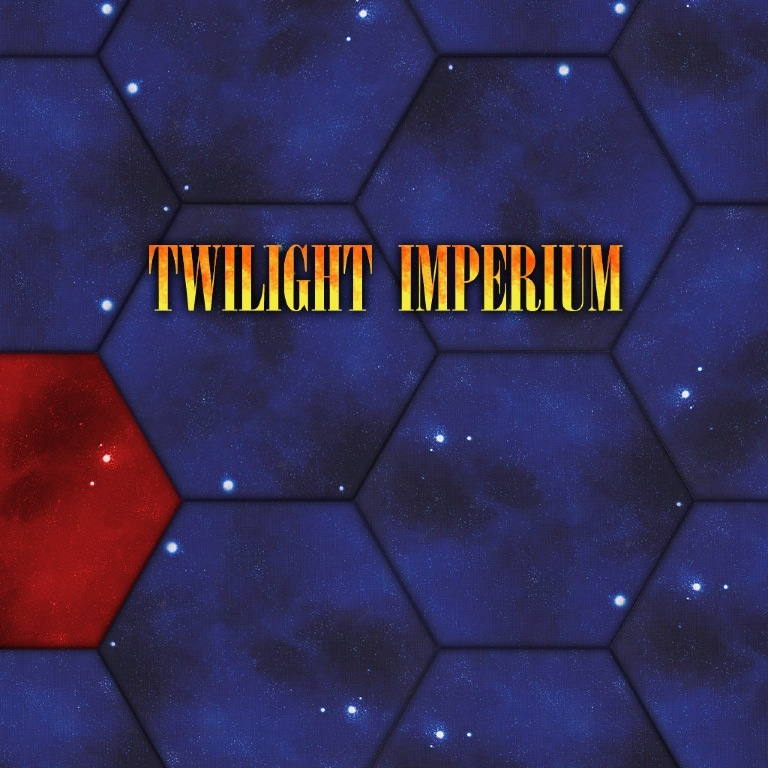
\includegraphics[height=\paperheight, width=\paperwidth]{pic945263}}} % Image background
\centering
\vspace*{10cm}
\par\normalfont\fontsize{1}{1}\sffamily\selectfont
\textbf{Twilight Imperium 3rd Ed.}\\
{\LARGE\textcolor{yellow}{All in One Manual}}\par % Book title
\vspace*{1cm}
{\Huge\textcolor{yellow}{ A Game by Christian T.Petersen}}\par % Author name
\endgroup
%----------------------------------------------------------------------------------------
%	COPYRIGHT PAGE
%----------------------------------------------------------------------------------------

\newpage
~\vfill
\thispagestyle{empty}

%\noindent Copyright \copyright\ 2014 Andrea Hidalgo\\ % Copyright notice

\noindent \textsc{The all in one live Twilight Imperium 3rd edition Manual}\\

% \noindent \textsc{github.com/LaurethTeX/Clustering}\\ % URL



\noindent Originally edited by Oigelb (http://boardgamegeek.com/user/Oigelb).
Many Corrections by kiminoboku (http://www.boardgamegeek.com/user/kiminoboku).\\ 
This version is also edited by Rafaelolg (http://boardgamegeek.com/user/rafaelolg)\\
\\

\noindent Game Design (all editions): Christian T. Petersen\\
Additional Development (3rd edition): Greg Benage\\
Game Design for the Expansions: Corey Konieczka and Christian T. Petersen\\
Editing: Greg Benage\\
Graphic Design: Brian S. Schomburg, Andrew Navaro and Michael Silsby, Tom Garden and Mark Molnar\\


% License information
\noindent \textit{TWILIGHT IMPERIUM is a trademark of Fantasy Flight Publishing, Inc. Copyright 1997-2011 Fantasy Flight Publishing, Inc. All Rights Reserved. The products, or any parts thereof, may not be reproduced without the publisher's consent.} % Printing/edition date


\begin{table}[!htbp]
\centering
\caption{Versions of this document}
\label{docversions}
\begin{tabular}{|l l l|}
Version & Date        & Comment                                                                          \\
\hline
1.0     & 18.Jan 2012 & First Release                                                                    \\
1.1     & 22.Feb 2012 & Updated to FAQ 2.4                                                               \\
1.2     & 28.Feb 2012 & Corrected FAQ about Flagships and TypeIV Drive and Nano Tech                     \\
1.3     & 24.Apr 2012 & Corrected pagination and player diagram for 7-8 players                          \\
1.4.1   & 26.Aug 2014 & Corrected Front Page                                                             \\
1.4.2   & 06.Dec 2014 & Corrections and houserules from kimioboku                                        \\
1.4.3   & 11.Jul 2015 & Minor Corrections, thx to ZaRaZa                                                 \\
1.4.4   & 21.Jul 2015 & Minor Corrections, thx to ZaRaZa, Kelanen and Arael                              \\
1.4.5   & 17.Oct 2015 & Minor Corrections (FAQ 2.5: Remove systems in 8-player game) and minor graphics. \\
1.5     &  2017       & Move all content to latex . \\
\end{tabular}
\end{table}
%----------------------------------------------------------------------------------------
%	TABLE OF CONTENTS
%----------------------------------------------------------------------------------------

\chapterimage{head1.png} % Table of contents heading image

\pagestyle{empty} % No headers

\tableofcontents % Print the table of contents itself

%\cleardoublepage % Forces the first chapter to start on an odd page so it's on the right

\pagestyle{fancy} % Print headers again

%----------------------------------------------------------------------------------------
%	CHAPTER 1
%----------------------------------------------------------------------------------------

\chapterimage{ti05_preview.jpg} % Chapter heading image
\chapter{Introduction}

\section{The Object of the Game}\index{Objective}
To win a game of TWILIGHT IMPERIUM ("TI"), players seek to accumulate a total of 10 victory points by achieving objectives and carefully choosing helpful strategies. The game ends when one player gains his 10th victory point or immediately after any other game-ending condition applies (see later).

\section{Notations}\index{Notations}

This document has rules that are specific to to optional parts of the game. To make easy to trace and find wich parts you can/want to use this document will use the following notation.

\textbf{Base game} rules will be in the main text.

\begin{SEbox}
Rules and options from \textbf{Shattered Empire Expansion} will be marked with this blue box.
Or just a \SEf{a blue text}.
\end{SEbox}


\begin{STbox}
Rules and Options from the \textbf{Shards of the Throne Expansion} (SoT) will be marked this red box. 
Or just a \STf{red text}
\end{STbox}

\begin{FFGbox}
Online Rules and Options from the FFG-Website will be marked with this green box. 
Or just \FFGf{a green text}.
\end{FFGbox}

\begin{HRbox}
House-Rules and Options (from boardgamegeek.com and ti3wiki.org etc.) with this gray box or just \HRf{a gray text}.
\end{HRbox}



\section{Game Contents and Preparations}\index{Game Contents and Preparations}

\begin{figure}[h]
    \centering
    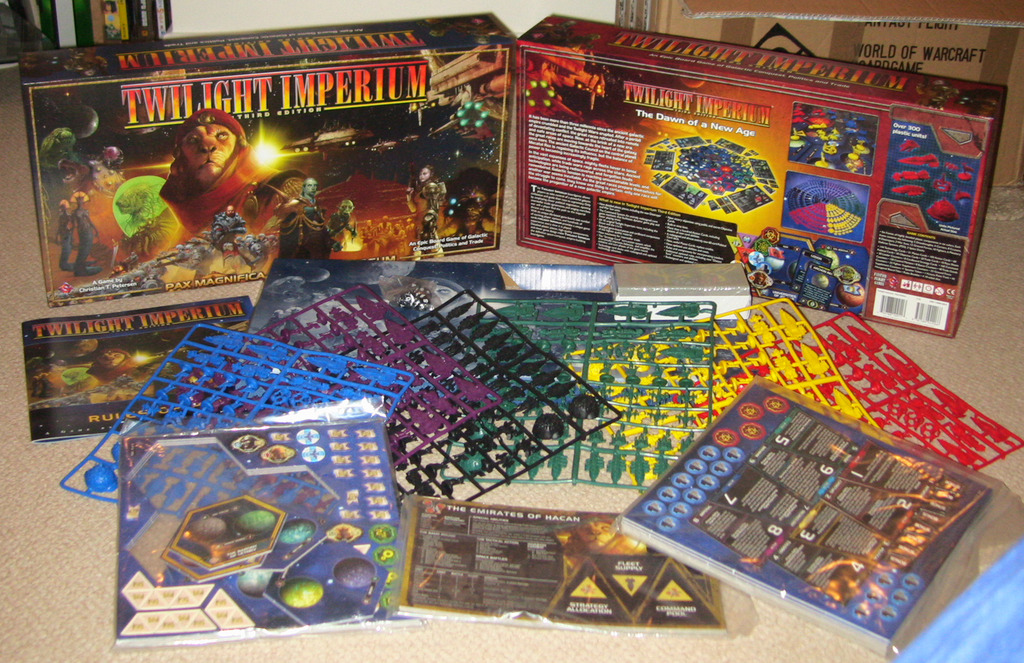
\includegraphics[width=\textwidth]{components.jpg}\\
    \caption{Twilight Imperium 3 straight out of shrinkwrap. image by MattDP@bgg https://boardgamegeek.com/image/222231}
    \label{fig:game_compoments}
\end{figure}


\begin{itemize}
\item 6 \SEf{8 in SE} frames of highly detailed plastic components in 6\SEf{8} colours. Each frame contains the following:
\begin{itemize}
\item 5 Dreadnoughts
\item 4 Carriers
\item 8 Cruisers
\item 8 Destroyers
\item 2 War Suns
\item 12 Ground Forces
\item 10 Fighters
\item 6 Planetary Defense Systems (PDS)
\item 3 Space Docks
\item \STf{1 Flagship}
\item \STf{4 Mechanized Units}
\end{itemize}
\item 256 Technology Cards (32 each in eight decks separated by colour) (24x6 in Base Game, \SEf{28x8 in SE}, \STf{32x8 in SotT}) (\SEf{3 Replaced Techs x 6 in SE})
\item \SEf{34 Race-specific Technologies Cards} (\SEf{14 SE}, \STf{22 SoTT}), (\STf{2 Replaced in SotT})
\item \STf{3 Race-specific Technology Tokens}
\item \STf{17 Flagship Cards}
\item 34 Trade Cards (2 each for 17 races)
\item 51 Leader Counters (3 each for 17 races)
\item 272 Command Counters (16 each for 17 races)
\item 289 Control Markers (17 each for 17 races)
\item \STf{51 Representative Cards (3 each for 17 races)}
\item 17 Race Sheets (10 Basegame, 4 Shattered Empire, 3 Shards of the Throne)
\item 86 Hexagonal Board Tiles (43 from Base Game, 28 from Shattered Empire, 15 Shards of the Throne) 
\item 91 Planet Cards (51 Base Game, 28 SE, 12 SotT)
\item \SEf{16 Facility Cards (8 Colonies, 8 Refineries)}
\item 170 Action Cards (103 Base Game, \SEf{40 Shattered Empire}, \STf{34 SotT}) (7 Replaced Cards (\SEf{5 SE}, \STf{2 SotT}))
\item 110 Political Cards (60 Base Game, 32 Shattered Empire, 19 SotT) (1 Replaced Card)
\item 68 Objective Cards (Secret and Public) (30 Base Game, 28 Shattered Empire, 10 Preliminary SotT)
\item 16 Mercenary Cards
\item 40 Promissory Note Cards
\item 20 Cardboard Strategy Cards (8 Base Game, 8 Shattered Empire, 1 Variant Strategy Card from SE, 3 Variant Strategy Cards from SotT)
\item 8 Bonus Counters
\item 64 Trade Goods Counters (40 Base Game, 12 SE, 12x3 SotT)
\item 51 Fighter Supplement Counters (23x1, 28x3), (23 Base Game, 12 SE, 16 SotT)
\item 51 Ground Force Supplement Counters (23x1, 28x3) (23 Base Game, 12 SE, 16 SotT)
\item \SEf{12 Shock Troop Tokens}
\item \SEf{12 Space Mine Tokens}
\item \SEf{2 Mecatol Custodian Tokens}
\item \SEf{8 Artifact Tokens}
\item \SEf{1 High Alert Token}
\item \SEf{3 Worm Hole Tokens}
\item 66 Domain Counters (44 Base Game, 22 SE,)
\item 15 Space Domain Counters
\item 16 Mercenary Tokens
\item \SEf{8 Unit Reference Cards} (\STf{8 new in SotT})
\item 1 Speaker Token
\item 1 Victory Point Track
\item This rules booklet
\item 4 10-sided dice (note that in TI, the "0" result represents the number "10")
\end{itemize}

\begin{STbox}
\subsubsection{Components of the Scenario “Fall of the Empire”}
\begin{itemize}
\item 1 Race Sheet (the Lazax)
\item 16 Lazax Command Counters
\item 17 Lazax Control Counters
\item 2 Scenario Strategy Cards
\item 34 Agenda Cards
\item 1 Lazax Objective Card
\item 7 Scenario Objective Cards
\item 2 Lazax Trade Agreements
\item 31 Treaty Cards
\item 1 Variant Mecatol Rex Hexagonal Board Tile
\end{itemize}
\end{STbox}

\begin{SEbox}
\subsection{Shattered Empire Components}\index{Shattered Components}
\subsubsection{The Shattered Empire Icon}


\includegraphics[]{se_icon.png}\\

All the cards in this expansion are marked with the \emph{Shattered Empire} symbol on their fronts, to allow you to easily separate them from your base \emph{Twilight Imperium} game.

\subsubsection{Replacement Cards for Base Game}

Several replacement cards for the Twilight Imperium 3rd Edition base game are included in this expansion. Some of these cards have been revised to correct errata, while others have been revised to work better with this expansion. To use the replacement cards, simply remove the original cards from their appropriate decks and replace them with the new versions. The replacement cards are:
\begin{itemize}
\item TECHNOLOGY CARDS
\begin{itemize}
\item 6 Advanced Fighters (1 in each colour)
\item 6 Micro Technology (1 in each colour)
\item 6 Assault Cannon (1 in each colour)
\end{itemize}
\item ACTION CARDS
\begin{itemize}
\item 4 Direct Hit Cards
\item 1 Ruinous Tariff Card
\end{itemize}
\item POLITICAL CARDS
\begin{itemize}
\item 1 Open the Trade Routes Card
\end{itemize}
\end{itemize}
\end{SEbox}

\begin{STbox}
\subsection{The Shard of the Throne Components}\index{Shattered Components}

\subsubsection{The Shard of the Throne Icon }


\includegraphics[]{st_icon.png}

All the cards included in this expansion are marked with the \emph{Shards of the Throne} symbol on their fronts (pictured above), to allow you to easily separate them from your base \emph{Twilight Imperium} game.
\subsubsection{Replacement Cards for Base Game}
\begin{itemize}
\item ACTION CARDS
\begin{itemize}
\item 1 Ghost Ship Card
\item 1 Star of Death Card
\end{itemize}
\item RACE-SPECIFIC TECHNOLOGY CARDS
\begin{itemize}
\item 1 Bioptic Recyclers Card
\item 1 Berserker Genome Card
\end{itemize}
\end{itemize}

\end{STbox}

\section{Component Overview}
We will here summarize the various components of TI, so that you may recognize them while reading these rules.

\subsection{Map Hexes}
Before every game of TI, players will create a unique game board by connecting the provided hexagon map pieces. Each individual piece is called a "system." The systems of TI each represent an area of space, its planets, and/or other elements of interest. Systems that contain an interior yellow outline are \textbf{Home Systems} from which the great races hail. Systems containing an interior red outline are \textbf{Special Systems} (such as Asteroid Fields) governed by special rules.

\begin{SEbox}There are 28 new system tiles in SE, including Ion Storms (a new type of Special System). Hope’s End, the imperial training ground, is also among the new systems. One of the new systems is the Wormhole Nexus (WN), which is easily distinguished by its non-hexagonal shape. Use of this system is optional, and when this rulebook refers to systems, the WN should be excluded unless stated otherwise.
\end{SEbox}

\begin{STbox}
There are 14 new system tiles in SotT, including a Gravity Rift (a new type of Special System) and new Home Systems. A variant version of Mecatol Rex, used only in the Fall of the Empire scenario, is also among the new systems.
\end{STbox}
\subsection{Plastic Game Units}
The detailed plastic pieces of TI (collectively called "units") represent the military personnel, shipyards, defensive systems, and spaceships that players will command. Units not employed on the game board are kept in a player’s reinforcement area.

\subsection{Planet Cards}
Representing the multitude of planets in TI, Planet Cards are used by players to indicate ownership over each individual planet and are "exhausted" (turned face down) when their owner "spends" the planets' resources or influence.

\subsection{Technology Cards}
At the beginning of the game, each player receives an identical Technology Deck (separated by colour) consisting of 24 \SEf{(28 with SE)} \STf{(32 with SotT)} technology advances. Throughout the game, when a player purchases (or otherwise acquires) a technology, the corresponding Technology Card is taken from his deck and placed face-up before him. 
\subsection{ Action Cards}
The Action Cards of TI provide players with a variety of helpful events, manoeuvres, bonuses, and other advantages. Players receive Action Cards throughout the game by a variety of activities.


\subsection{Political Cards}
Often the representatives of the great races must meet in the hallowed halls of the Galactic Council on
Mecatol Rex to debate, deliberate, and enact policy for the custodial imperial charter. When a player executes the primary ability of the Political Strategy Card during the Action Phase (see later), he must draw and resolve the top card of the Political Deck. Each Political Card contains an \textbf{agenda} that all players must vote upon. The effects of an agenda can range from a minor formality, to a major change in the very structure of the game.

\subsection{Objective Cards (Public and Secret)}
In order to win TI, players need to accumulate 10 victory points. The primary way for players to receive such is by qualifying for the requirements of an Objective Card. The victory points provided by Public Objective Cards are attainable by all players, whereas those from Secret Objective Cards are individual to each player.
\begin{SEbox}
    
The new sets of Stage I and Stage II Public Objectives can optionally be used instead of the original Objective deck. These cards tend to focus more on military conflict than the original set. Also provided are 3 new Secret Objectives, to be mixed in with the original set.
Finally, Special Objectives have been included for use with two new optional rules: Artifacts (detailed on page 65) and the Voice of the Council option (detailed on page 68).
\end{SEbox}
\begin{STbox}
Preliminary Objective Cards optionally start players with easier objectives worth 1 victory point each. Also provided are Scenario Objective Cards, only used in the Fall of the Empire scenario (including a special Lazax Objective Card).
\end{STbox}
\begin{STbox}
    
\subsubsection{The Secret Objective Deck}
Some cards and rules in this expansion refer to the Secret Objective deck. This deck consists of any Secret Objective not in play. Instead of placing unused Secret Objective cards in the box, simply place them in the play area. When a player fulfils a Secret Objective card, it is removed from the game (and not shuffled back into this deck).
\end{STbox}

\subsection{Trade Cards}
Each race has two Trade Contract cards which they can use to form trade agreements with other players. Each Trade Card has a numerical trade value which varies from race to race.

\subsection{Strategy Cards}
Each of the eight cardboard Strategy Cards represents a powerful short-term strategy. During the Strategy Phase of each game round, each player will select one Strategy Card and must later use its primary ability. Each Strategy Card also enables an important secondary ability that other players may execute after the primary ability is resolved.
\begin{SEbox}
    
SE  features a new set of eight variant Strategy Cards, with a white background, that favours different strategies than the original set. In addition, there is a High Alert token for use with the new Warfare II Strategy Card. The variant Imperial Strategy Card, with a black background, may optionally be used with the original set of Strategy Cards.
\end{SEbox}
\begin{STbox}
SotT  features variant Political, Assembly, and Trade Strategy Cards. Two Strategy Cards only used for the “Fall of the Empire” scenario are also included (Civilization and Industry, s. page 76).
\end{STbox}

\subsection{Bonus Counters}
After all players have selected a Strategy Card during the Strategy Phase, there will (in a six-player game) be two Strategy Cards remaining in the common play area. Before the Strategy Phase ends, the two remaining Strategy Cards both receive a Bonus Counter that is placed on top of the Strategy Card itself. A player that later selects such a Strategy Card will be able to use the Bonus Counter to receive an additional Command Counter or Trade Good.


\subsection{Command Counters}
The Command Counter in TI is the abstract but integral resource representing the domestic mandate,
budget, organization, logistics and preparedness of your race. When a player receives a Command Counter from his reinforcements, he must place it in either the Fleet Supply area, Strategy Allocation area, or Command Pool area on his Race Sheet. In order to execute tactical actions (such as moving, building, or initiating combat on the board), take advantage of the secondary abilities of Strategy Cards, or manage his fleets, a player must wisely allocate and spend Command Counters.

\subsection{Control Markers}
At the beginning of the game, each player is provided with a generous number of flag-shaped Control Markers, each bearing the insignia of that player's race. The Control Markers are used to represent a race wherever appropriate, such as on the Victory Point Track, on successfully achieved Objective Cards, and (most often) to indicate ownership of planets.

\subsection{Trade Good Counters}
These counters represent the wealth and rewards of interstellar commerce. They are primarily obtained by active trade agreements while the Trade Strategy Card is being executed. A player's Trade Goods can be used as a direct substitute for either resources or influence, and are frequently used as currency among players to pay for bribes or other considerations.

\subsection{Victory Point Track}
The Victory Point Track is used to indicate each player's accumulation of victory points. Note that the main side of the Victory Point Track has spaces numbered from 0 to 10, whereas the reverse side is numbered 0 to 14. The reverse side is be used with the optional rule “The Long War” found on page 57.

\subsection{Speaker (First Player) Token}
This token is claimed each round by the player who selects the Initiative Strategy Card during the Strategy Phase. The player who controls the Speaker Token always chooses the first Strategy Card during the next Strategy Phase.

\subsection{Ground Force and Fighter Unit Supplement Tokens}
The Ground Force and the Fighter units are the only units in the game that players may purchase unlimited quantities of. All other unit types are limited to the figures provided with the game. The Fighter and Ground Force supplement tokens represent the extra Fighter and Ground Force units that players may add to their forces.

\subsection{Race Sheets}
Enclosed in your game, you will find 10 (\SEf{14 with SE}, \STf{17 with SotT}) large cardboard sheets, each representing one of the great races of the TI universe. After selecting a race to play, each player receives the corresponding Race Sheet, which provides each player with specific information for his race as well as helpful game information tables. The Race Sheet is also used for keeping track of a player’s active Command Counters and Trade Goods.
\begin{STbox}
A race sheet for the Lazax is also included in SotT. The Lazax race is only used in the “Fall of the Empire” scenario (see page 76). Cards and Markers are also provided for this race.
\end{STbox}
\begin{SEbox}    
\subsection{Race-Specific Technologies}

Each of the 17 races now has one Race-Specific Technology. These optional Technology cards may only be acquired by the appropriate race (see page 64). \STf{In SotT there is a second race-specific Technology per Race included.}

\subsection{Facility Cards}
These cards represent refineries and colonies that players may build on a planet to increase the planet’s resources or influence value. See page 67 for details.

\subsection{Unit Reference Cards}
The unit reference cards provide players with an image of each unit type and its game stats.

\subsection{Shock Troop Tokens}
Shock Troops represent battle-hardened, veteran Ground Forces. These special Ground Forces are much more powerful and have special rules governing them (found on page 65).

\subsection{Space Mine Tokens}
With the new Space Mines option, Cruisers have the ability to deploy space mines. Ships moving into a system that contains space mines could be destroyed before combat. See details on page 66.

\subsection{Mecatol Rex Custodian Tokens}
These tokens represent guardians of Mecatol Rex. Their optional use is described on page 68.

\subsection{Artifact Tokens and Objective Cards}
These tokens represent four ancient relics of power that are hidden somewhere through out the galaxy. Each Artifact also has a corresponding Special Objective card worth 1 Victory Point to its controller., See details on page 65.

\subsection{Wormhole Tokens}
Special Wormhole tokens have been included for use in optional map setups.

\end{SEbox}

\begin{STbox}
\subsection{Agenda Cards}
These cards replace the Political Card deck when playing the “Fall of the Empire” scenario.

\subsection{Flagship Cards}
Each of the 17 races now has the ability to build its own Flagship, a powerful warship with unique race-specific abilities. These optional ships may only be built by the appropriate race (see page 70).

\subsection{Mercenary Cards}
These cards represent Mercenaries that players may hire using the new Trade III Strategy (s. page 72).

\subsection{Promissory Note Cards}
Players can now offer Promissory Notes in the Galactic Council. These new cards are used with the new Political II and Assembly II Strategy Cards (see page 74).

\subsection{Representative Cards}
Each of  the races has 3 Representatives that players may choose from to send to the Galactic Council. These optional cards are used with the new Political II and Assembly II Strategy Cards (see page 13).

\subsection{Treaty Cards}
These cards are only used in the “Fall of the Empire” scenario. Players can make alliances with each other using these cards.

\subsection{Space Domain Counters}
These new counters are used with the Final Frontier option. See page 70 for more information).

\subsection{Mercenary Tokens }
These tokens mark the locations of Mercenaries (a new type of unit) on the board. They are double-sided to display whether the Mercenary is in space or on a planet. The appropriate battle value for each Mercenary is also displayed on each side.

\subsection{Race-specific Technology Tokens }
Special Tokens have been included for use with the Ghosts of Creuss’ and the Embers of Muaat’s special abilities.

\end{STbox}
\chapterimage{rexbanner.jpg}
\chapter{Setup}\index{Setup}
\begin{figure}[h!]
    \centering
    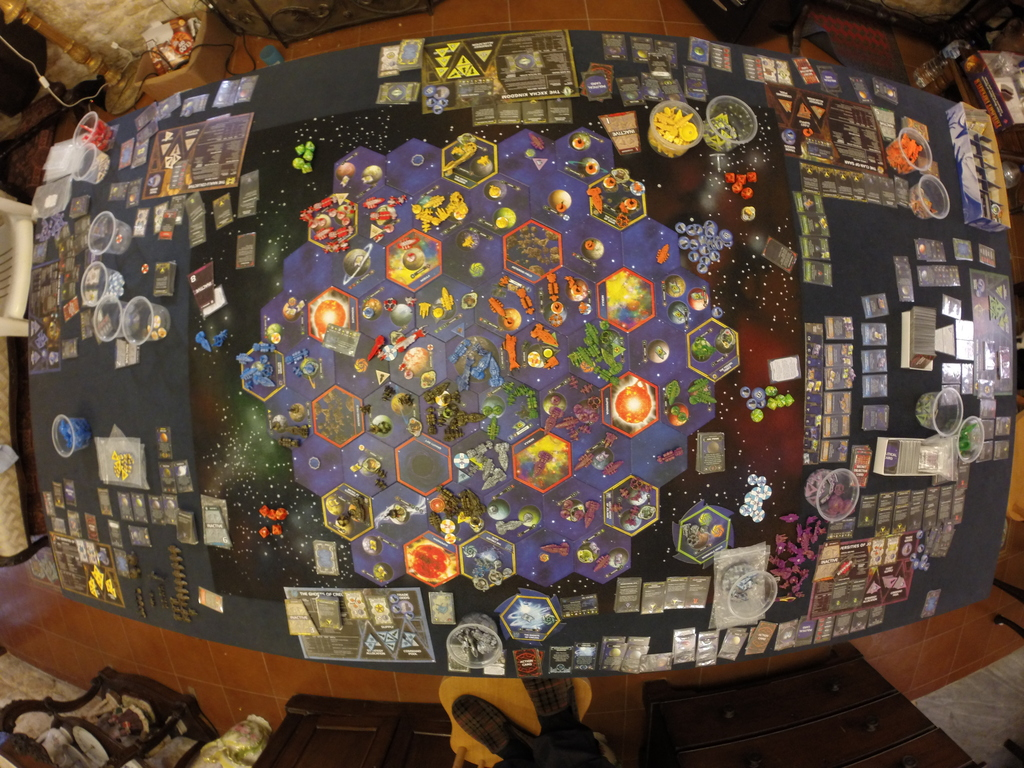
\includegraphics[width=\textwidth]{gametable.jpg}\\
    \caption{8 player game. Photo by tintii@bgg https://boardgamegeek.com/image/2355207}
    \label{fig:game_table}
\end{figure}

\section{Number of Players}
These rules are written assuming that you will be playing TI with 6 players. TI plays just as well with
fewer players, and rules for playing with 3-8 players are provided on page 53 of this rules set.


\section{Setup and Play Area Organization}

\begin{figure}[!h!]
    \centering
    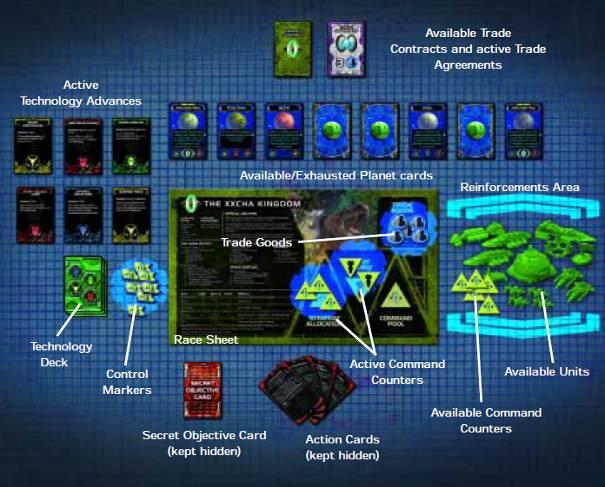
\includegraphics[width=\textwidth]{playarea.jpg}\\
    \caption{Suggested Player Area}
    \label{fig:play area}
\end{figure}

\begin{figure}[!h!]
    \centering
    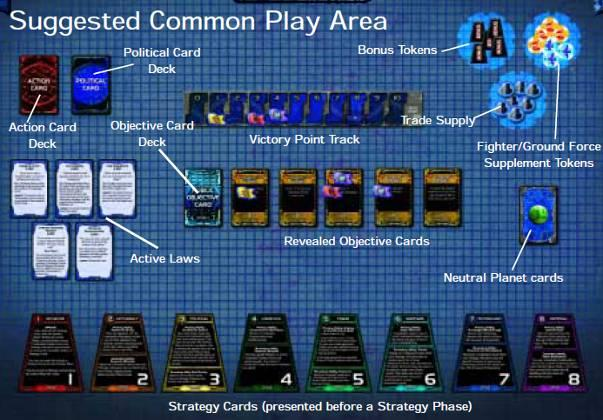
\includegraphics[width=\textwidth]{commonplayarea.jpg}
    \caption{Suggested Common Play Area}
    \label{fig:play area}
\end{figure}

Before you start playing, follow the steps below:
\begin{enumerate}
\item Separate the 10 Home Systems from the other hexagonal game-board pieces. Randomize the Home Systems face down and allow every player to draw one at random. This process determines which race a player will control throughout the game. All players then take the Race Sheet, Control Markers, Trade Cards, and Command Counters corresponding to their race.
\item Each player selects one of the six available colours and takes the plastic units and Technology Deck corresponding to that colour.
\item Find an area of the table that is convenient for all players to reach. Designate this space the "common play area." Then shuffle the Action Card deck and the Political Card deck and place them separately in the common play area. Also place the Fighter and Ground Force Supplement Counters in the common play area.
\item Each player takes the individual Planet Cards corresponding to the planets of his Home System and places these face up in his play area. Place the remaining Planet Cards, representing the neutral planets at the start of the game, in the common play area.

\item Place all the Trade Goods Counters in a single pile (the "Trade Supply") in the common play area.
\item Now place the 8 Strategy Cards side-by-side in numerical order with their "active" side up, prominently in the common play area.
\item Create the Objective Deck, by following the directions in the "Preparing the Objective Cards" sidebar. Do not forget to place the unused Secret and Public Objective Cards back in the box, while allowing no players to look at them.
\item Now place the Victory Point Track in the common play area and place one Control Marker for each player in the space marked "0."
\item Players must now create the game board (or “galaxy”). Please read and carry out the instructions for doing so in the "Setting up the Galaxy" sidebar on page 15 before proceeding.
\item After the galaxy has been created, all players place their "setup units" (as indicated by their Race Sheets) on their Home Systems. If a Home System contains several planets, any Space Dock, Ground Forces, and PDS may be placed among them according to the player’s wishes.
\item All players then find and place their "Starting Technology" cards face up in their respective play areas. All players now take their starting Command Counters from their reinforcements, placing them on their Race Sheets as follows: \textbf{2 Command Counters in the Strategy Allocation area, 3 Command Counters in the Command Pool area, and 3 Command Counters in the Fleet Supply area (with the "Fleet" side up)}.
\end{enumerate}


\subsection{Reinforcements}
Every player maintains a “reinforcement” area consisting of his unused plastic units and Command Counters. Whenever a player builds a unit, it is taken from his available reinforcements and thereafter placed on the board. (An exception to this is the Fighter and Ground Force Supplement counter, see later). Whenever a player receives a new Command Counter, it is taken from his available reinforcements and placed in one of the three appropriate boxes on his Race Sheet (Command Pool, Fleet Supply, or Strategy Allocation).

\subsection{Preparing the Objective Cards}
Before the game begins, the Secret Objective Cards must be distributed and the Public Objective Deck properly prepared. First separate all the Objective Cards into the three different types: Secret Objectives, Public “Stage I” Objectives, and Public “Stage II” Objectives. Then proceed to the following:

\begin{enumerate}
\item Shuffle the 10 Secret Objective Cards and deal a random card face down to every player. All players should read their Secret Objective Card and then place the card face down in their play area. A player is never allowed, for whatever reason, to show an opponent his Secret Objective Card. Place the remaining Secret Objective Cards back in the box, allowing no player to look at them.
\item Now take the 10 Stage II Public Objective Cards and remove the “Game Over” card. Shuffle the remaining 9 Stage II cards and draw 3 random cards (at all times keeping them hidden from all players). After drawing the 3 random cards, take the “Game Over” card and shuffle it with the 3 randomly-chosen cards. You should now have 4 randomized Stage II Public Objective Cards, one of which is the “Game Over” card. Place these 4 cards face down in a stack in the common play area. Place the remaining Stage II cards back in the box, allowing no player to look at them.
\item Then shuffle the 10 Stage I Public Objective Cards and draw 6 random cards. Place the 6 cards on top of the 4 Stage II cards, now forming a single deck of 10 Public Objective Cards in the common play area. This deck always consists of 6 random “Stage I” cards on top of 4 random “Stage II” cards (one of which is the “Game Over” card). This deck is the “Public Objective Deck.”
\end{enumerate}

\begin{STbox}   
     It is important that the unused Objective Cards (Secret, Public Stage I \& II) are placed back in the box so they remain hidden from players both before and during the game. Otherwise, experienced players would be able to deduce which objectives are in play before they are revealed.

\end{STbox} 

\emph{You are now ready to start the game.}



\chapterimage{twilight-imperium.jpg}
\chapter{Rules}\index{Rules}

\section{Objective of the Game}\index{Objective}
To win a game of TWILIGHT IMPERIUM ("TI"), players seek to accumulate a total of 10 victory points by achieving objectives and carefully choosing helpful strategies. The game ends when one player gains his 10th victory point or immediately after any other game-ending condition applies (see later).

\section{Creating the Galaxy}

\begin{figure}[!h!]
    \centering
    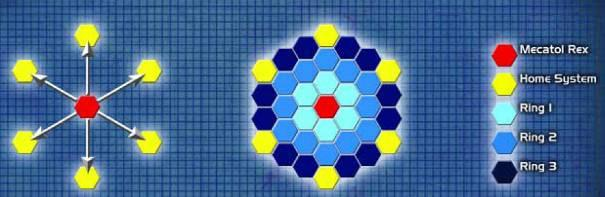
\includegraphics[width=\textwidth]{creating_galaxy.jpg}
    \caption{Galaxy creation schematics}
    \label{fig:galaxycreation}
\end{figure}
TI uses a unique game board consisting of multiple hexagon pieces (“systems”) that are brought together in a unique combination at the beginning of every game. Players build the galaxy by following these steps:

\begin{enumerate}
\item After all players have drawn their Home Systems, find the Mecatol Rex system and place it in the middle of the table. Then randomly determine one player to be “first player. Give the “Speaker“-Token to the first player. He then shuffles the remaining 32 systems, \emph{randomly removes two systems} (by placing them back in the box without looking at them), and deals five systems, face down, to every player. Players may look at their dealt systems but should not show them to the other players.
\item The first player now selects one of the sides of Mecatol Rex, and drags his Home System about two feet towards himself in a straight line away from the chosen side (see diagram). Then the player to his left does the same, etc., until all players have chosen a side and placed their Home Systems on the table (note that the sixth player must chose the last remaining side of Mecatol Rex). Players should now shift their seating around the table to best accommodate their Home System placement.
\item Then players, in clockwise order, starting with the first player, begin creating the galaxy by placing, one at a time, a single system face up adjacent to the Mecatol Rex system. After the first ring around Mecatol is completed, players continue to place systems in the second ring until that is completed, and then finally proceed to the third ring.
\end{enumerate}

When all the systems are placed, the galaxy is finally created. The following rules apply to placing systems:

\begin{itemize}
\item A system cannot be placed in the second ring before the first ring surrounding Mecatol Rex has been completed. Likewise, a tile cannot be placed in the third ring before the second ring is completed (see diagram).
\item As soon as the correct placement for your Home System becomes available, connect your Home System to the galaxy at its fixed spot (which is exactly 3 systems out from the chosen side of Mecatol Rex, see diagram). Connecting your Home System is automatic and does not cost you a placement “turn.”
\item You may not place a Special System (with an inner red border) adjacent to another Special System, unless you have no other option.
\item The order of placement switches counter clockwise after all players have placed a round of tiles and yet again clockwise after that, etc. This in effect will make the player, who placed the last system, place the first system in the next round (thus actually placing two systems in a row). Example of turn order: P1, P2, P3, P4, P5, P6, P6, P5, P4, P3, P2, P1, P1, P2…
\item If you placed a system that did not contain a planet during your last placement, you must, if able, place a system that \emph{does} contain a planet during your next placement. If you are unable to do so, you must reveal your remaining systems to the other players to prove this. Then place one of your available systems.
\end{itemize}

When creating the board, the actual shape of the galaxy and the position of Home Systems will differ depending on the number of players. If you are playing a game with less than six players, please consult the optional rules on page 53 of this rules booklet.

\begin{SEbox}
    \subsection{Game Setup with the New Systems from the Expansion Shattered Empire}
    Due to the addition of many new systems, players will need to remove more random systems before setting up the galaxy than specified in the base game.

The first player should place these systems back in the box during setup without looking at them.

Remove the following systems instead of the systems specified on page 53 of the original rulebook:
\begin{itemize}
\item 3 Players: Remove 7 empty, 6 Special, and 18 Regular Systems (with planets).
\item 4 Players: Remove 4 empty, 5 Special, and 14 Regular Systems (with planets).
\item 5 Players: Remove 4 empty, 5 Special, 14 Regular Systems (with planets), and 1 random system.
\item 6 Players: Remove 4 empty, 5 Special, 14 Regular Systems (with planets), and 2 random systems.
\end{itemize}
\subsection{Larger Galaxy Games}
With five or six players, players may wish to set up an additional outer ring. To do this, fewer tiles are removed during setup.
\begin{itemize}
\item 5 Players: Deal out every tile, so that each player has 11 tiles. Then create the galaxy as normal. (Unlike the standard 5-player setup described on page 32 of the original rules, no random system is placed adjacent to Mecatol Rex.)
\item 6 Players: Remove 1 random hex and then deal out the rest, so that each player will have 9 tiles.
\end{itemize}

Then create the galaxy as described on page 8 of the original rulebook. However, in step 3 of “Creating the Galaxy,” continue placing systems until there are 4, rather than just 3, rings around Mecatol Rex.
\end{SEbox}


\begin{STbox}
\subsection{Game Setup with the New Systems from both Expansions}

Due to the addition of many new systems, as well as the systems introduced in Shattered Empire, players now have more options when setting up the galaxy. Instead of removing the systems specified on page 53 of the original rulebook, players create three piles of systems; one pile of Special Systems (all systems with red borders), one pile of empty systems (all systems with no planets), and one pile of Regular Systems (all remaining non-Home Systems). Without looking at the tiles, players deal a number of random systems into a galaxy pile and shuffle it. All remaining tiles are returned to the game box without looking at them. Players then use the systems in this galaxy pile to create the galaxy (following all normal setup rules).

\begin{itemize}
\item 3 Players: Shuffle together 3 Special, 5 empty, and 16 Regular Systems.
\item 4 Players: Shuffle together 4 Special, 8 empty, and 20 Regular Systems.
\item 5 Players: Shuffle together 4 Special, 8 empty, and 20 Regular Systems. Randomly remove 1.
\item 6 Players: Shuffle together 4 Special, 8 empty, and 20 Regular Systems. Randomly remove 2.
\SEf{
\item *7 Players: Shuffle together 9 Special, 12 empty, and 34 Regular Systems, randomly remove 2
\item *8 Players: Shuffle together 9 Special, 12 empty, and 34 Regular Systems, randomly remove 3
\item *5 Players (Larger Galaxy): Shuffle together 9 Special, 12 empty, and 34 Regular Systems.
\item *6 Players (Larger Galaxy): Shuffle together 9 Special, 12 empty, and 34 Regular Systems. Randomly remove 1.\\
\item *Requires the Shattered Empire expansion.}
\end{itemize}
\end{STbox}

\section{The Game Round}
After you have finished setting up the game, players will begin playing the game by starting with the
\emph{Strategy} Phase of the first game round. TWILIGHT IMPERIUM is played over a consecutive number of game rounds with each round consisting of the following phases:

\begin{itemize}
    \item The Strategy Phase
    \item The Action Phase
    \item The Status Phase
\end{itemize}

After every Status Phase, if no player has yet declared victory, simply begin another game round starting with another Strategy Phase, etc. In this way the game continues, repeating the three phases above, until a player has achieved 10 victory points or until another game-ending condition is met.

Victory points are generally claimed during the Status Phase as players fulfil the requirements printed on the Public and Secret Objective Cards. In order to meet these various objectives, players must seek to expand their empires, forge alliances with other races, negotiate for the best outcome during the Galactic Council, and choose the optimal Strategy Cards during the Strategy Phase.


\subsection{ Strategy Phase}
During every Strategy Phase, each player must choose one available Strategy Card from the common play area (The chosen Strategy Card grants its player a special ability during the upcoming Action Phase.) At the beginning of every Strategy Phase, there are 8 possible Strategy Cards (or "strategies") that players may choose from. These are: Warfare, Political, Trade, Initiative, Imperial, Logistics, Diplomacy, or Technology.

Not only does the Strategy Card provide an important ability, but it also determines the \emph{order of play} (as indicated by its number; see the text box on page 20 for more information on the order of play).
At the beginning of every Strategy Phase, the player who controls the Speaker Token (the "Speaker") may choose the first Strategy Card from the common play area.

When selecting a Strategy Card, a player simply chooses and takes an available Strategy Card from the common play area and places it before him (with the "active" side facing up).

That card is now no longer available for selection by the other players.

After the Speaker has picked his Strategy Card, the other players, in clockwise order from the Speaker, each select one of the remaining Strategy Cards. In this way every player will pick an available Strategy Card before the Action Phase begins. Note that being farther clockwise from the Speaker gives a player an increasingly limited choice of Strategy Cards (i.e., the player to the immediate right of the Speaker will only have three cards to choose from).

After all players have selected a Strategy Card, there will be two cards remaining in the common play area. The Speaker places a \emph{Bonus Counter} on the two remaining unchosen Strategy Cards.

In this way, should a Strategy Card not be picked for several consecutive rounds, multiple Bonus Counters will accumulate on it.
The presence of Bonus Counters makes a Strategy Card more attractive in subsequent rounds.

When a player selects a Strategy Card that contains one or more Bonus Counters, that player may immediately exchange each Bonus Counter for either a Trade Good or a Command Counter (either of which is immediately placed on the player's Race Sheet).

After all players have chosen their Strategy Cards and the Bonus Counters have been placed on the remaining cards, the Strategy Phase ends and the game proceeds to the Action Phase.

Note that the last player to claim the Speaker Token will keep the Speaker Token until another player selects the Initiative card during a future Strategy Phase.

\subsection{Action Phase} % (fold)
\label{sub:action_phase}

The Action Phase forms the heart of TI. It is during the Action Phase that players will execute the special abilities of their Strategy Cards, produce new units at their Space Docks, conquer new planets, and move their fleets into battle.

rn order would be the player who selected the Diplomacy Strategy.


The Action Phase is resolved over a number of \emph{player turns} in which each player may take a \emph{single action}. Each player turn is taken in the order of play (see text box on page 21), with players one after the other taking one action to complete their turn. After the last player in the order of play has taken his turn, play returns once more to the first player in the order of play who may take an action, followed by the second player, and so on. In this way, players keep taking one action at a time, following the order of play, until all players have passed and the Action Phase ends.

\subsubsection{Order of Play}
Each Strategy Card has an Initiative Number printed near its top. This number represents what place in the order of play its owner will be. Thus, the player who has the Initiative Strategy card is always first, followed by the player who controls the Diplomacy Strategy card, etc. The order of play, as dictated by the Strategy Cards, is as follows:
\begin{enumerate}
    \item Initiative Strategy
    \item Diplomacy Strategy
    \item Political Strategy
    \item Logistics Strategy
    \item Trade Strategy
    \item Warfare Strategy
    \item Technology Strategy
    \item Imperial Strategy
\end{enumerate}

When the turn order advances to an unchosen Strategy Card in the common play area, simply skip it and proceed to the next number. If, for example, no player picked the Initiative Strategy card during the Strategy Phase, the first player in the tu

A player that is currently in the process of taking his turn (i.e., action) is called the \emph{active player}. When it is a player's turn to take an action, he must execute one of the following:
\begin{itemize}
\item Strategic Action
\item Tactical Action
\item Transfer Action
\item Pass 
\end{itemize}

% subsubsection the_player_action (end)

\subsection{Strategic Action} % (fold)
\label{sub:strategic_action}
A player must, at some point during the Action Phase, execute a Strategic Action (except for the player holding the Initiative Strategy Card, who has no Strategic Action).

When a player chooses to take his Strategic Action, he first reads and then resolves the \emph{Primary Ability} as printed on his Strategy Card. After the active player has finished resolving the Primary Ability, the other players, in \emph{clockwise order from the active player}, may each spend one Command Counter from their Strategy Allocation area on their Race sheet to execute the \emph{Secondary Ability} of the current Strategy Card.

\begin{STbox}
    \emph{Special Exception}: Players do not have to spend a Command Counter from their Strategy Allocation area when executing the Secondary Ability of the Logistics Strategy Card.
\end{STbox}

The active player \emph{may never} execute the Secondary Ability of his own Strategy Card.
After all players have completed (or passed on) the Secondary Ability, the active player's Strategy Card is flipped over onto its "Inactive" side and the player action is over.
A player may only take one Strategic Action per round. Likewise, a player may only execute any given Secondary Ability once (but a player may, if he has a sufficient number of Command Counters in his Strategy Allocation area, participate in the Secondary Ability of several Strategy Cards).
The initiative number on each Strategy Card only determines the order of play. Players may execute
their Strategic Action at a time of their choosing, regardless of its initiative number.  It is likely, for example, that the player holding the Trade Strategy will take his Strategic Action before the player holding the Logistics Strategy, even if the Logistics Strategy has a lower initiative number. Details for each specific Strategy Card can be found on page 88.  

\subsection{Tactical Action} % (fold)
\label{sub:tactical_action}

The Tactical Action is the primary function for engagement on the game board. It is during a Tactical
Actions that you will move your fleets on the board, engage in space battles, transport your Ground Forces to new planets, build new units, etc. 
The process of taking a Tactical Action always follows the "Activation Sequence" below:


\emph{The Activation Sequence}
\begin{enumerate}
\item Activate a system
\item Move ships into the system
\item PDS fire
\item Space Battle
\item Planetary Landings
\item Invasion Combat
\item Produce Units
\end{enumerate}

Except for the first step (the activation itself), each individual step of the Activation Sequence is only resolved if the condition for its resolution applies or is initiated by the active player. 

A player, for example, may activate a system to produce new units there during step 7, but does not necessarily have to move any ships into the system during step 2. Or, a player may activate a system and move ships into the system, but if the system contains no enemy ships, there is no Space Battle during step 4, etc.
On the other hand, step 2 through 7 cannot be executed unless preceded by the initial activation.

If a player has no Command Counters left in his Command Pool, he cannot take a Tactical action, and therefore not move ships, fight battles, produce units, etc.
\begin{FFGbox}
    \emph{“Friendly“ and “Enemy“}

When the cards and rules of TI refer to a “friendly” unit or planet, it refers to a unit or planet belonging to you (i.e., a single player). Although you may have an alliance or be personally friendly with another player, for the purposes of TI rules, only your own units and planets are “friendly”.

When the rules refer to an “enemy” planet or unit, it refers to any unit or planet not controlled by you (i.e., controlled by any other player). Even though you may have an alliance with another player, and even though you may consider the other players your personal friends, for the purposes of TI rules, the units and planets of other players are considered “enemy.”

\end{FFGbox}

\subsubsection{Activation Sequence in Detail}
Below, each step in the Activation Sequence is described in detail. Rules for how to resolve Space Battles and Invasion Combat can be found on pages 27 through 30.

\begin{description}
\item [1 - Activate a System] Take an available Command Counter from your Command Pool and use it to activate a system by placing the Command Counter directly on a system (place the counter face-up so that your race's insignia is showing). You cannot activate a system if one of your Command Counters has already been placed in the system (by a prior activation or by other means). You can, however, activate a system that contains one (or more) Command Counters belonging to other races (you may ignore their presence). A system that contains a player's Command Counter is considered to have been \emph{activated} by that player.  

\emph{In summary}: When the TI rules and cards refer to an "activated" system, this means a system that contains a Command Counter of the player in question. 
As a general rule, for purposes of activation and movement, a player can ignore the presence of Command Counters on the board belonging to other players.

This means, for example, that every race can activate a specific system. In such a case, that system would contain a Command Counter from each race and would be considered “activated” by all players.  Although the Command Counters on the board belonging to other players do not limit where you may activate a system, it can be helpful to study which systems an opponent has activated, since those system cannot be activated again by that player this round, nor can his ships in his activated systems move. 

\item [2 -  Move Ships into System] 
After you have activated a system, you may move friendly ships (within movement range) into the activated system. \emph{Only movement into the activated system is allowed.}

The rules for moving ships during a Tactical Action are as follows:
\begin{itemize}
    \item Every ship (except for Fighter units, which move with Carriers or War Suns) has a movement value found on the unit table located on every player's Race Sheet. A movement of "1" indicates that a ship can move from its current system into an adjacent system. A movement of 2 indicates that the ship may move up to two systems from its current system, etc.
    \item A Carrier/War Sun may pick up Ground Force and PDS units at any stage during the movement step (before, during, and even in the activated system itself). Ground Force and PDS units aboard a Carrier, however, cannot be "dropped off" by the Carrier until the Planetary Landing step of the Activation Sequence. \emph{If the last Ground Force unit on a planet is picked up by a Carrier, the owner of the planet must place a Control Marker on the planet to indicate that he controls it}. There are some exceptions to this rule (See P.45 for Ground Force and P.46 for Carrier).
    
    \item A ship is never allowed to move through a system occupied by enemy ships (except Fighters). The only way to enter a system that contains enemy ships is to activate that system itself.

    \item A ship may not move if it is located in a system that already has been activated by the active player (i.e., contains a friendly Command Counter placed prior to the current activation). It therefore follows that, once a ship has moved into an activated system, the very Command Counter used for the activation will prevent the ship from moving again during the same round. Ships \emph{are allowed to move through} systems containing friendly Command Counters.
\end{itemize}
Certain effects by Strategy or Action Cards can remove Command Counters from the board, allowing systems to be activated again by the same player (and allowing any friendly units in such a system to move again, etc).

\emph{In summary}: Only ships that can actually enter the activated system may move. 
Ships that are out of movement range, that need to pass through a system containing enemy units, or are in a system already activated, may not move. Remember, any ship moving must always end its movement in the system that was just activated. See the detailed graphical example of a Tactical activation and movement on page 24.


\item[3 - PDS Fire]
After the active player has finished moving his ships into the activated system, enemy PDS in range may fire at the active player's fleet. For every "hit," the activating player must remove a casualty from the fleet (note that Dreadnoughts and War Suns can take one "Damage" before they are destroyed, see page 52). After enemy PDS units have fired, any PDS in range owned by the active player may then fire at enemy ships in the activated system. For more details on PDS units, see page 48.

\item[4 - Space Battles]
First determine whether a Space Battle will occur in the activated system.
If the active player has moved one or more ships into a system that contains ships controlled by an opponent (even a Fighter) a Space Battle \emph{must} be initiated between the two players.

A Space Battle will continue until only one player has ships remaining in the system. If a Space Battle is initiated, the active player is the \emph{Attacker} and the player whose ships were in the system before activation is the \emph{Defender}.  For complete rules of how to resolve a Space Battle, please see the “Space Battles” section on page 27]

\item [5 - Planetary Landings] 
After any Space Battles are completed, the active player may now commence Planetary Landings by landing Ground Force and PDS units from his Carriers onto planets in the activated system.

If a system contains multiple planets, the active player may split any landing forces between them in any way he sees fit, but may not change his mind once the Invasion Combat step begins. There are three types of Planetary Landings:
\begin{description}
    \item [Friendly Landing] A player lands units on a planet already under his control. Simply add the new units to the ones already there, if any.

    \item [Neutral Landing] A player lands units on a neutral planet (i.e., a planet controlled by no other player). After landing at least one Ground Force unit on the neutral planet, the active player takes the corresponding Planet Card from the Planet Deck and places it exhausted in his play area. Note that only a Ground Force unit can take over a planet. If a PDS unit lands alone on a neutral or enemy planet, it is immediately destroyed.

    \item[Hostile Landing (also called an "Invasion")] A player lands units on a planet containing one or more of an enemy player’s Ground Force units. This will result in an Invasion Combat during the Invasion Combat step.
\end{description}

If a player lands units on a planet that is controlled by an opponent, but does not contain any enemy Ground Forces, the planet falls without resistance. The invader simply removes the opponent’s Control Marker and takes the corresponding Planet Card from the opponent, placing it exhausted into his play area.

\item [6 Invasion Combat] After planetary landings, should any planet contain Ground Forces of two different players, that planet must now engage in Invasion Combat.  If a system has several planets engaged in Invasion Combat, the battles are resolved one-at-a-time in the order decided by the active player.

\emph{Landing PDS units with an Invasion:} The invading player is allowed to land PDS units with his Ground Forces during the Planetary Landings step. Such PDS units do not participate in Invasion Combat, nor can they be taken as a combat casualty. If the last invading Ground Force unit is destroyed during Invasion Combat, all invading PDS are immediately destroyed with no further effect. 
Details for how to resolve Invasion Combat are found in the “Invasion Combat” section on page 30.

\item[7 - Produce Units]
As the final step of a Tactical Action, the active player may produce new units at one or more friendly Space Docks in the activated system. During this step, it is also possible for the active player to produce a new Space Dock unit on an eligible planet in the activated system (provided that the planet has been under the player’s control for the entire round). See more information on how to produce units under the Space Dock on page 44 concluding a Tactical Action.

After resolving the steps of the Activation Sequence (Activate a system, Movement, PDS fire, Space Battles, Planetary Landings, Invasion Combat, and Production), the Tactical Action is over and the opportunity to take an action proceeds to the next player in the order of play.

\end{description}
\begin{FFGbox}
    \subsubsection{Definition of a Fleet}
    For the purposes of the TI rules and cards, a fleet is defined as all spaceships (Fighters, Cruisers, Carriers, Dreadnoughts, Destroyers, and War Sun units) controlled by one player in one system at any given time.
\end{FFGbox}


\subsection{Transfer Action} % (fold)
\label{sub:transfer_action}
The Transfer Action is a simple reorganization of units that cannot be effectively handled by the Tactical Action. The Transfer Action simultaneously activates two \emph{adjacent systems that only contain units belonging to the active player} and allows units in either system to simultaneously move between the two systems. In addition to this movement, the active player may also produce units in one of the two systems if a Space Dock is present in either. The process of taking a Transfer Action always follows the steps of the \emph{Transfer Sequence}:
\begin{enumerate}
    \item Activate two systems
    \item Movement between systems
    \item PDS Fire
    \item Planetary Landings
    \item Production (in one system)
\end{enumerate}
Below, each step of the Transfer Sequence is described in detail:

\begin{description}
    \item[1 - Activate two Systems]
    After announcing a Transfer Action, the active player takes one Command Counter from his Command Pool and activates a system by placing the Command Counter upon it. Then the active player takes a Command Counter from his \emph{reinforcements} and activates another system \emph{adjacent} to the one just activated. Both activated systems must contain at least one unit controlled by the active player and must contain absolutely no enemy units (including Ground Forces and PDS).

    \emph{Reminder}: When "activating a system" the active player places a Command Counter physically on the system itself (with his race insignia facing up). It is never possible for a player to activate a system that is already activated (i.e., already contains one of his Command Counters).

\item [2- Movement]
    The active player may now move friendly ships \emph{between} the two activated systems. As during a Tactical Action, Fighters, PDS, and Ground Force units must be transported by Carrier/War Sun.

\item[3 - PDS Fire]
After the active player has finished moving, \emph{enemy} PDS in range may fire at the active player's fleets in the activated systems. PDS units that are in range of both activated systems may fire at only one of the systems, not both.

\item 4 - Planetary Landings]
During this step, any Ground Force and PDS units onboard Carriers in the activated systems may land on friendly planets in their system. Note that during a Transfer Action you may only land forces on friendly systems, not neutral planets or planets containing an enemy Control Marker.

\item 5 - Production]
The active player may now produce units at his Space Docks in \emph{one} of the activated systems (but not both).

\end{description}


\subsection{Passing}     % (fold)
\label{sub:passing}

If a player does not wish to take any additional actions, he may choose to pass. 

A player is only allowed to pass if he has already taken his Strategic Action (except for the player who controls the Initiative Strategy, who has no Strategic Action). All players must therefore, at some point during the Action Phase, take their Strategic Action (and thereby allow other players to execute the Secondary Ability of their Strategy Card). 

After a player has passed, he is no longer allowed to take any additional actions this round. 
When it normally would have been his turn in the order of play, simply skip him, and proceed to the next player.

\begin{STbox}
    A player, who has passed, is allowed to execute the Secondary Ability of Strategy Cards that are resolved later during the phase.

    \emph{Example: After taking several actions, including his Strategic Action, the Xxcha player decides to pass. After doing so, the game goes on for several additional cycles until the Letnev player decides to take his Strategic Action. 
    After the Letnev has resolved the Primary Ability of the Strategy Card, the other players, including the Xxcha, are allowed to execute its Secondary Ability.}
\end{STbox}
% subsection passing (end)

\subsection{End of the Action Phase} % (fold)
\label{sub:end_of_the_action_phase}

The Action Phase continues, repeating the order of play, until all players have passed. 

This could potentially result in a remaining player taking several consecutive actions, while all other players, having passed, must wait for him to finish his actions. Once all players have passed, the game proceeds to the Status Phase.

\subsection{Example of Activation and Movement} % (fold)
\label{sub:example_of_activation_and_movement}
In the example above, the N’orr player has just initiated a Tactical Action during the Action Phase. As the first step, he takes a Command Counter from his Command Pool and places it on the system occupied by the Xxcha fleet and planet.
After activating the system, he proceeds to the second step in the Activation Sequence. As the N’orr player may now move ships into the activated system, his movement options are as follows:
\begin{enumerate}
\item The Dreadnought has a movement rate of 1. Since the activated system is 2 spaces away, it is too far preventing the Dreadnought from moving into the activated system.

\item Although these two Cruisers are in two different systems, they each have a movement rate of “2,” which allows them to reach the activated system. The two Cruisers may move into the activated system. The top Cruiser will move through a system that contains another N’orr Command Counter, which is perfectly legal.

\item This fleet of one Destroyer, one Carrier and four Fighters are all within movement range, and may all move into the activated system. If he wishes, the N’orr player may split the fleet and only move some of the ships (although the Fighters should stay with the Carrier).

\item These two Destroyers are within movement range of the activated system, but their system was already activated earlier by the N’orr player. This prevents them from moving to the activated system. 

\item This N’orr Cruiser is within movement range to reach the activated system, but it cannot move through the Supernova or through the system containing two Xxcha Destroyers. This prevents the Cruiser from moving to the activated system.
\end{enumerate}

After moving units into the activated system (being careful not to exceed his Fleet Supply) the N’orr player will engage in Space Battle against the Xxcha fleet there.

\begin{figure}[h]
\centering
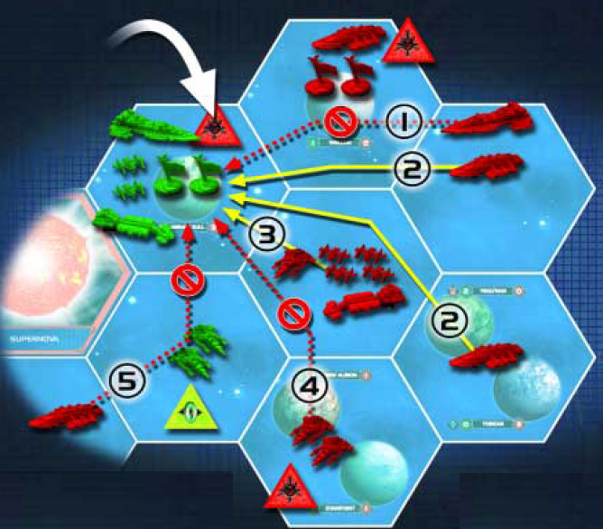
\includegraphics[width=0.87\textwidth]{activation_example.png}
\caption{ Example of Activation and Movement}
\label{fig:example_activation}
\end{figure}

\subsection{Status Phase} % (fold)
\label{sub:status_phase}

The Status Phase, when compared to either the Strategy or Action Phase, is a straightforward experience. It is during the Status Phase that many of the game functions are "reset," such as players refreshing Planet Cards, discarding Command Counters from the board, etc. It is also during the Status Phase that players may gain victory points by meeting the requirements of a Public and/or Secret Objective Card. To resolve the Status Phase, follow the Status Sequence below:
\subsubsection{The Status Sequence}
\begin{enumerate}
    \item  Qualify for Public/Secret Objective Cards
\item Repair Damaged Ships
\item Remove Command Counters
\item Refresh Planet Cards
\item Receive 1 Action Card and 2 Command Counters
\item Redistribute Command Areas
\item Return Strategy Cards
\end{enumerate}

\subsection{Qualify for public/secret Objectives} % (fold)
\label{sub:qualify_for_public_secret_objectives}        
In the order of play, each player may announce that he has met the requirements of one face-up Public Objective Card and/or his Secret Objective Card.
After a player announces that he has met the objectives of a face up Public Objective Card, he must prove to his opponents that his claim is valid.
After doing so, the player places one of his Control Markers on the claimed Objective Card (indicating that he has claimed that objective), and then advances his Control Marker on the Victory Point Track the appropriate number of spaces.
Once a player has received Victory Points for a specific Objective Card, he may not qualify for that Objective Card again.
In addition, if a player has met the requirements of his Secret Objective Card, he may now reveal the card, prove that its objectives are met, and then claim its victory points.

\emph{Important Exception: A player may never qualify for a Public or Secret Objective Card if he does not control all the planets in his Home System.}
% subsection qualify_for_public_secret_objectives (end)
% subsection status_phase (end)

% subsection example_of_activation_and_movement (end)
% subsection end_of_the_action_phase (end)
% subsection action_phase (end)
% That's how science is made, thinking and testing and thinking again, creating your own scientific method, comming up with hypothesis, learning what might work and what not, using your insticts. 

% Well, before comming here I didn't think like that, it was just all about being super productive and thinking about doing robots and all kinds of devices with sensors. I had some experience programming in C/C++, no computer science backgound and I had never had an astronomy course.

% This report was written in order to help someone to continue researching about data mining techniques applied in Astronomy, I explain how did I come up with the clustering techniques, my hypothesis, some tests and other ideas I have had, I hope this can help anyone and the research is continued. Anything you may need/questions do not hesitate to contact me, my e-mail address is: \emph{mrs.petzl@gmail.com}, also s part of my own documentation I created a GitHub page where you can download all the codes I programmed and find more information. The link to this page is: \url{https://github.com/LaurethTeX/Clustering}, from the \textsc{readme} file you can acces to all the pages, take your time to surf.
% %------------------------------------------------

% \subsection{References}\index{References}

% Since I found so much good information about pretty much everything I wanted to know about, I will just create a remark and let you know where you can find more specific information about, just like below.

% \begin{remark}
% For more information about the cosmological principle, review Chapter 1: Why Learn Astronomy?, page 10, from \textbf{21st Century Astronomy}, \textit{Hester | Smith | Blumenthal | Kay | Voss}, Third Edition, 2010.
% \end{remark}

% %This statement requires citation \cite{book_key}; this one is more specific \cite[122]{article_key}.


% %----------------------------------------------------------------------------------------
% %	CHAPTER 2
% %----------------------------------------------------------------------------------------
% \chapterimage{band1.png}

% \chapter{Discovering what to do...}

% \section{First ideas}\index{First ideas}
% So, now here you have your first astronomy picture, \footnote{For example purposes the image selected is a picture of M83 through a Wide H-alpha and [N II] filter. } what do you see?, it is a monochrome image, with different levels of brightness, slightly big (8500 x 5000), it looks like a lot of stars making a spiral.
% \begin{figure}[h]
%     \centering
%     
\includegraphics[width=0.77\textwidth]{ha-gray-conv-crp.jpg}
%     \caption{Picuture of the M83 galaxy, image taken from the WFC3 ERS M83 Data Products, http://archive.stsci.edu/prepds/wfc3ers/m83datalist.html}
%     \label{fig:awesome_image}
% \end{figure}

% How can we learn something about this image, quantize, get useful information? In the next subsections I will explain the first ideas.

% \subsection{Superpixel segmentation}
% The main concept of this is to cut an image into bigger neighborhood sections, so from an image that has $425x10^5$ pixels we can get maybe less than 500 superpixels, and then analyse separately those little sections and identify what kind of intersellar objects are they, look at image \ref{fig:super} it is a self-explanatory example of how a superpixel algorithm works.
% \begin{figure}[h]
%     \centering
%     
\includegraphics[width=0.37\textwidth]{combo.jpg}
%     \caption{Example of a superpixel algorithm}
%     \label{fig:super}
% \end{figure}
% There are many ways to do this and they vary according to color dimensions, methods and number of required superpixels and whether the algorithm is able to find borders and make pixel clasifications.

% \begin{remark}
% 	You can find some example test I tested with Matlab and with Python in this webapage: \url{https://github.com/LaurethTeX/Clustering/blob/master/Methods.md}, also there is a huge amount of information on th internet about this but here are two pages you might find useful:
%     \begin{itemize}
%     	\item Superpixel: Empirical Studies and Applications \\ \url{http://ttic.uchicago.edu/~xren/research/superpixel/}
%         \item Segmentation Algorithms in scikits-image \\ \url{http://peekaboo-vision.blogspot.ca/2012/09/segmentation-algorithms-in-scikits-image.html}
%     \end{itemize}
%     Also there is one article (from IEEE) I found about and might interest you, it's pure computer science,
%     \begin{itemize}
%     	\item Normalized Cuts and Image Segmentation \\ \url{http://www.cs.berkeley.edu/~malik/papers/SM-ncut.pdf}
%     \end{itemize}
% \end{remark}

% \subsection{PCA}

% Welcome to Astronomy where you will find more acronyms than words to mention something on articles, lots of fun!, well in this case PCA stands for Principal Component Analysis, the objective of this method is to reduce dimnensionality, tranform the data to another space where is can be manipulated and reduced, there are multiple examples of work that has been done in astronomy applying this technique.

% Therefor, the idea of applying this method is that if we have multiple-wavelenght images of the same target and transform them to PCA space then we will have less dimensionality and it will be easier to process all the data and fins valuable information.\footnote{Before I forget to mention, later I discovered that PCA is not comonly used for datamining preprocessing because it is hard to interpret the information in the output result. Imagine clusters of data on PCA space, how do you make sense to that?}

% \begin{figure}[h]
%     \centering
%     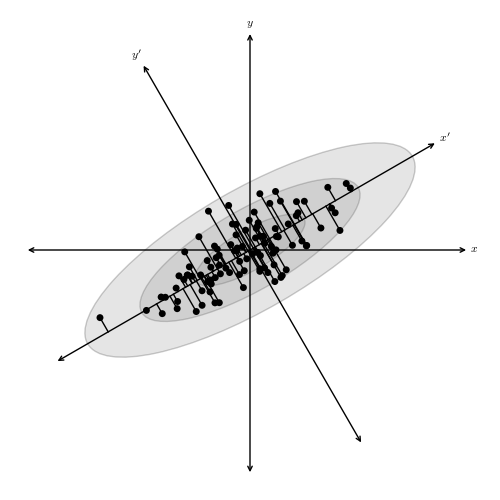
\includegraphics[width=0.37\textwidth]{fig_PCA.png}
%     \caption{A distribution of points drawn from a bivariate Gaussian and centered on the origin of $x$ and $y$. PCA defines a rotation such that the new axes ($x’$ and $y’$) are aligned along the directions of maximal variance (the principal components) with zero covariance. This is equivalent to minimizing the square of the perpendicular distances between the points and the principal components}
%     \label{fig:pca}
% \end{figure}

% \begin{remark}
% 	An example article, where they explain how to apply PCA on multi-wavelenght images and also mentions the pros and cons of using it.
%     \begin{itemize}
%     	\item Preserving Structure in Multi-wavelength Images of Extended Objects\\ \url{http://arxiv.org/abs/1101.1679v1}
%     \end{itemize}
%     There's a whole section that talks about this subject with a machine learning approach as a preprocessing step in this nice book,
%     \begin{itemize}
%     	\item Ivezi{\'c}, \v Z. and Connolly, A.J.
%          and Vanderplas, J.T. and Gray, A., \textit{Statistics, Data Mining and Machine Learning in Astronomy}, Princeton University Press, Princeton, NJ, 2014.
%     \end{itemize}
% \end{remark}

% \section{Hypothesis}\index{Hypothesis}
% Our data looks like the images on Fig.\ref{fig:cubes}, and it cointains data from let's say a determined galaxy at different wavelengths, if we assume that the galaxy contains various regions that relate to interstellar objects that can tell, how stars are formed, where, how stars die, where was a star, and other mysteries, I guess we can assume that those certain regions can be identified because they share similar characteristics, the ideas is to find how a galaxy is made from, its contents, apply the concept of the superpixel idea in 3D superpixels. 
% \begin{figure}[h]
% 	\centering
%     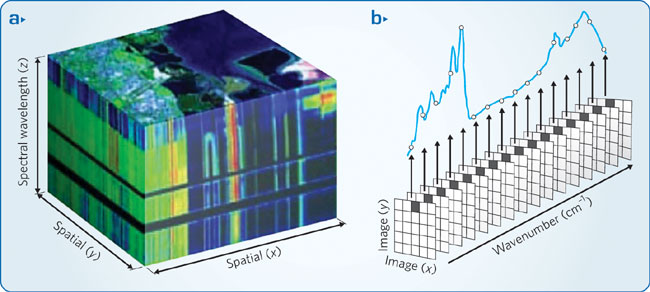
\includegraphics[width=0.57\textwidth]{nphoton.jpg}\hspace{1cm}
%     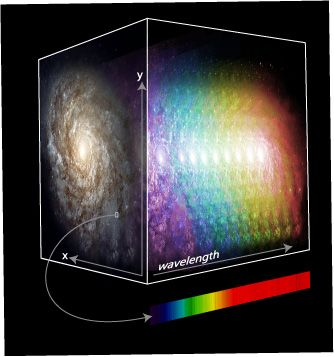
\includegraphics[width=0.27\textwidth]{data.jpg}
%     \caption{Illustrations of how a datacube looks like.}
%     \label{fig:cubes}
% \end{figure}

% Take the time to think about this, how the data looks like in 3D, how a star looks like in the datacube, imagine it, this is where ideas of how to tackle this problem come from.
% \begin{figure}
% 	\centering
%     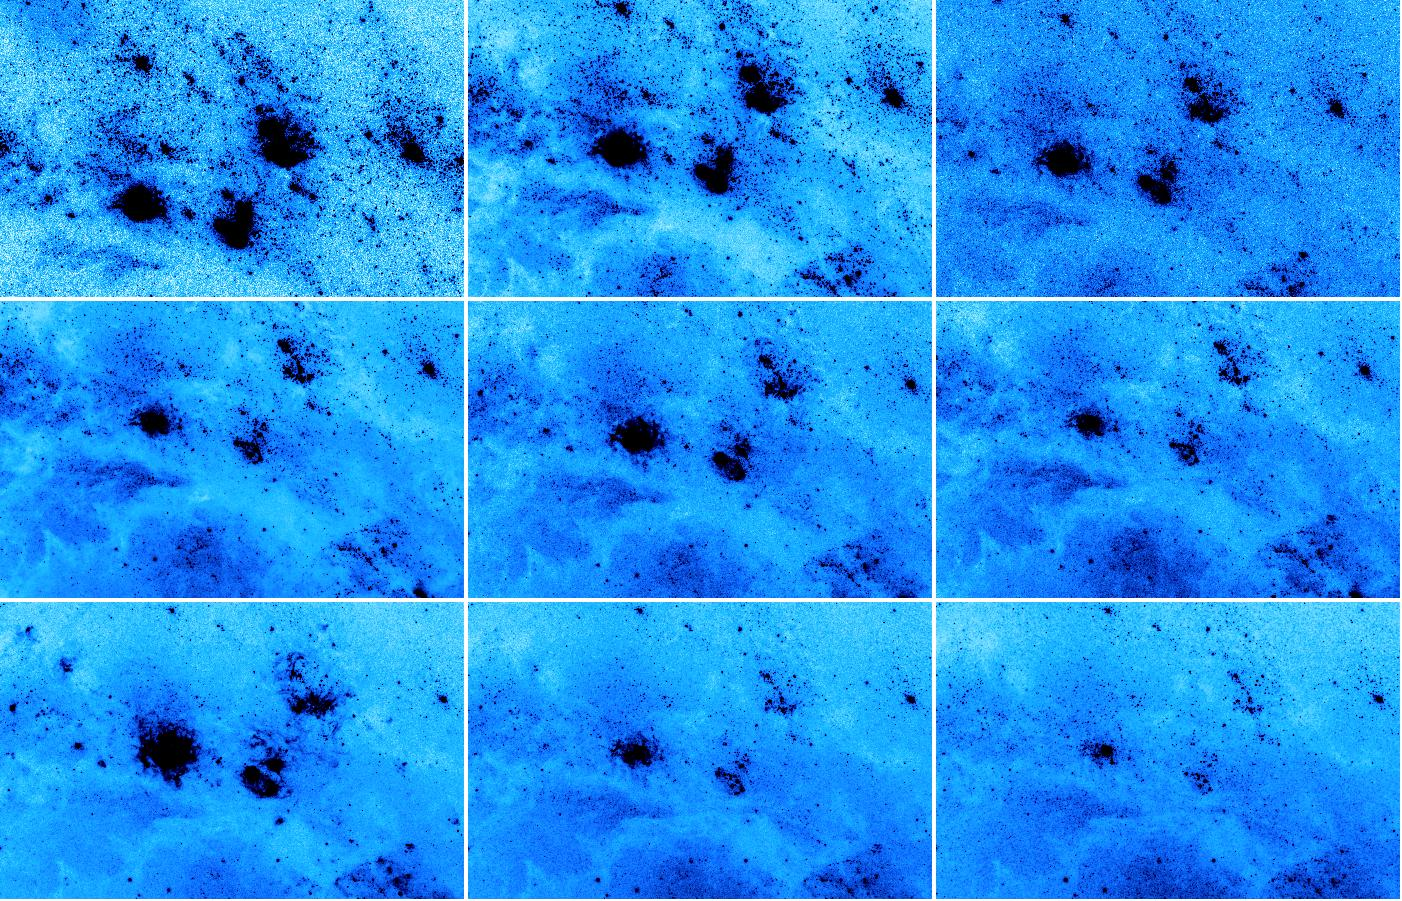
\includegraphics[width=0.87\textwidth]{nine.jpg}
%     \caption{Example of how an object can look in 9 wavelenghts}
%     \label{fig:nine}
% \end{figure}

% \subsection{Topics you should review}\index{Related topics}
% This will requere a lot of work, but hey it will be worthy and fun!
% \begin{itemize}
% 	\item Astroinformatics and computer science
%     	\begin{itemize}
%         	\item Data minig
%             \item Machine Learning
%             \item Big Data Analysis
%             \item Neural Networks
%             \item Visualization Resources
%         \end{itemize}
%     \item Statistics and Image Processing
%     	\begin{itemize}
%         	\item Probability Density Function
%             \item Point Spread Function
%             \item Full width at half maximum
%             \item Convolution
%         \end{itemize}
%     \item Interstellar medium and star formation
%     	\begin{itemize}
%         	\item HII regions
%             \item Planetary Nebulae
%             \item Supernova Remnants
%             \item Molecular Gas
%             \item All kinds of Nebulae (e.g. dark, refletion)
%             \item AGN's (Active Galactic Nucleus)
%         \end{itemize}
%     \item Astrophysics
%     	\begin{itemize}
%         	\item Units (light-years, parsecs)
%             \item World coordinate system
%         	\item Light
%             \item Telescopes
%             \item Stars and Stellar Evolution
%             \item Distance, Brightness, Luminosity
%             \item Galaxies
%         \end{itemize}
% \end{itemize}
% The GitHub page will certainly help you to understand why you need to learn about that, and where to find articles, wepages and books.
% \subsection{Downloading}
% First, let's equip ourselves with the basic software you will need in order to start then you may probably find other cool programs and later you will install them. There is also the possibility that your assigned computer will have them installed already but here is a brief description of what you can do with them, most of them are easy to use.

% \begin{description}
% 	\item[DS9:] It is a program that visualizes astronomy images in FITS format (don't worry if you recognize this format, it will be explained later), where you can easily manipulate them, read their headers, compare, look at regions, see their characteristics, make graphs, even movies. Well, depending on what you need to use later you will be finding all the functions, the best way is to click everywhere and find out what happens, also you can ask to your astronomy colleagues they will tell you all the perks, or if you like learning by yourself or you need someting specific check the documentation webpage. It is faily easy to install, just follow the instructions.
%     	\begin{description}
%         	\item[Download: ]\url{http://ds9.si.edu/site/Download.html}
%             \item[Documentation: ]\url{http://ds9.si.edu/site/Documentation.html}
%         \end{description}
%         The picture below shows (Fig.\ref{fig:screen}something cool you can do in DS9.
%         \begin{figure}[h]
%         	\centering
%     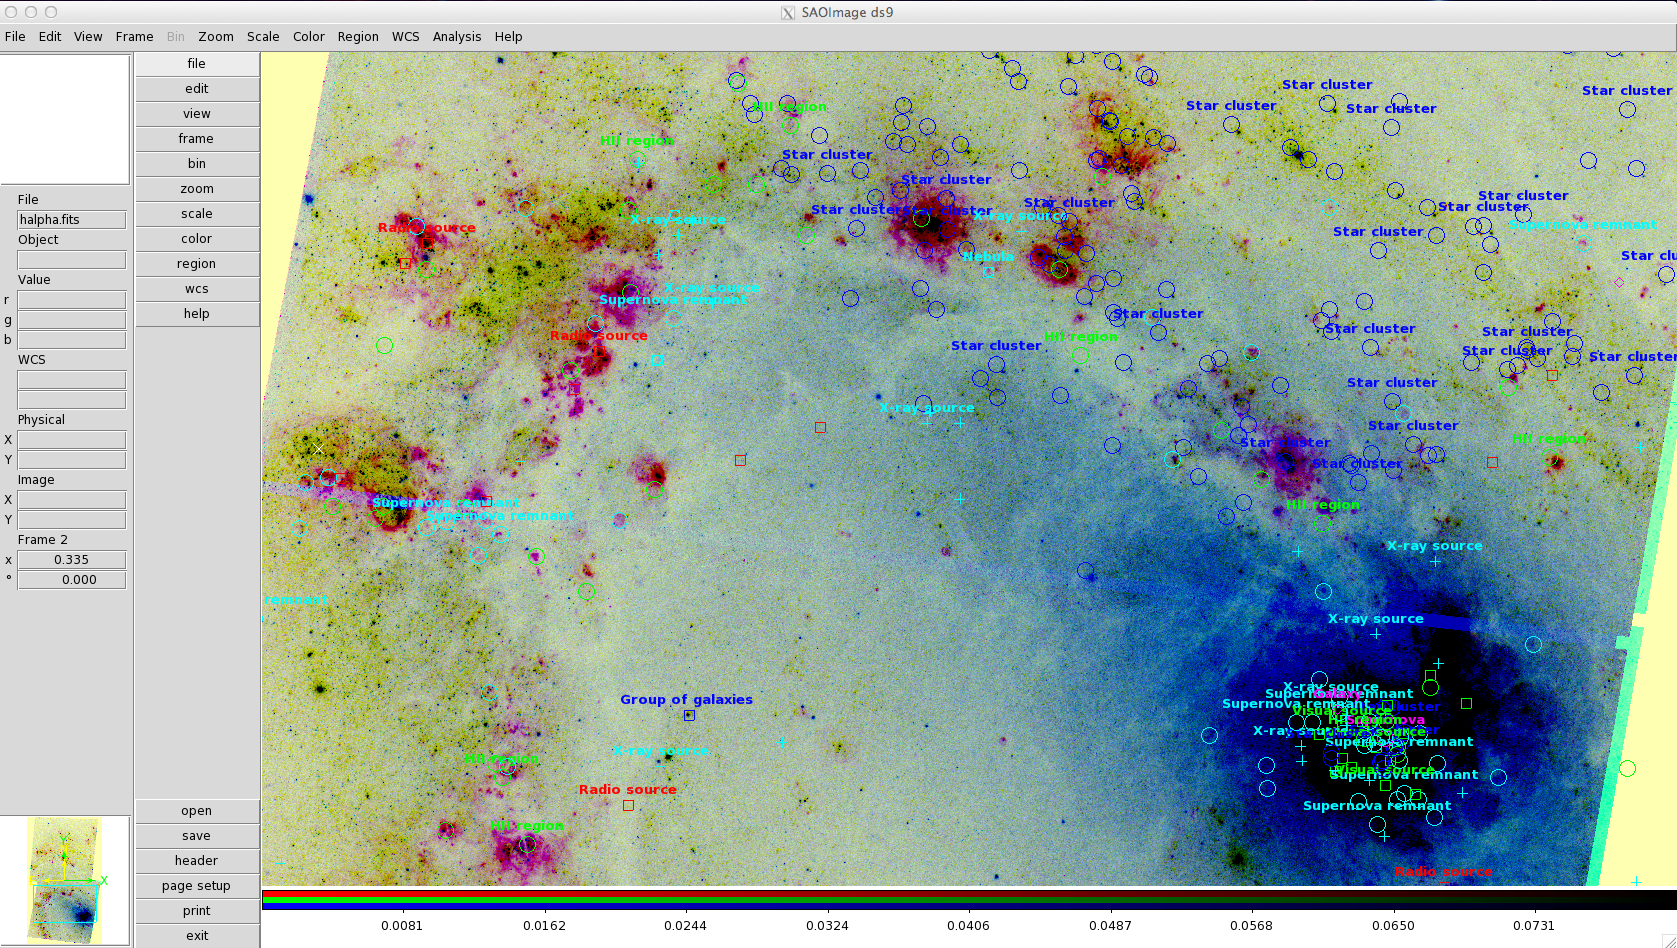
\includegraphics[width=0.87\textwidth]{Screenshot.png}
%     \caption{This is an RGB picure made from 3 independent FITS files, with a zscale and a region file overlaid from NED database, if you would like to learn more about this, or reproduce it, it is all explained in this webpage: \url{https://github.com/LaurethTeX/Clustering/blob/master/NEDtoREGION-FILE/KnownRegions.md}}
%     \label{fig:screen}
%         \end{figure}
        
%     \item[Python and a user interface: ]The most \emph{limitless} and user fiendly way to develop programs in Astronomy is using Python, there are many packages, modules, functions now available to help you in almost anything. Me, as an undergrad engineer I'm used to program on an user interface and not directly in a terminal. So, here I will explain you my own way of doing things.
    
%     I make my programs on the Canopy editor, it shows when and where you have programing error and warnings, and the interface is easy to learn, now to run, I open a terminal, go to the directory where my program is, type \verb|ipython| wait and then type \verb|run| \verb|myProgram.py|, and wait for the result.
    
%     Now there are a lot of fancier ways to work with \emph{Python}, you can program and test directly using \emph{IPython Notebook} on a web broswer or you can just go for the terminal, use \emph{nano} or \emph{vi} or the text editor you like and then run it by typing \verb|python| \verb|myProgram.py|. At this point is up to you, but hey here are some links to start and the packages/modules you should install.
    
%     \begin{description}
%     	\item[Interfaces or Development environments]\hfill
%         	\begin{itemize}
%             	\item PyCharm, it a development environment, just like CodeBlocks or NetBeans \url{http://www.jetbrains.com/pycharm/}
%                 \item Spyder, actually this is the interface that comes with the Python discritution Anaconda, you will get the Python districution and the intrerface. \url{https://store.continuum.io/cshop/anaconda/}
%                 \item Canopy, this is the one I mentioned before, it super easy to use and you can install packages with one click. \url{https://www.enthought.com/products/canopy/}
%             \end{itemize}
%         \item[Modules]\hfill
%         \\
%         In Python, modules are like the libraries in C, therefore, to use math, astronomy and computer science tools you need to install them. To learn whether you already have a module installed or not, type on \emph{iPython} \verb|import andreaModule|, if the output result is something like \verb|ImportError: No module named andreaModule|, you definitely don't have it installed. 
        
%         The strategy here to install packages it fairly easy, find their website, go to the download section and follow the instructions, almost all the packages are available on the Python Packaing Index and may be installed by running:
%         \begin{verbatim}
%         	pip install pyfits
%         \end{verbatim}
%         To learn how to use them check the documentation page, user manuals or their API's, if you have experience on object oriented programing it will be like running a new bike and if you don't, don't worry too much, Python was designed to be easy to program, just learn the rules of the game.
%         	\begin{itemize}
%             	\item Astropy, this package is the \emph{must have} of every astronomer, contains tools to handle coordinate systems, units, convolution.. well is better if you take a look at the webpage. \url{http://www.astropy.org/}
%                 \item Numpy, this package contains the math magic functions, linear algebra tools and the array management variables, make sure you learn all about \emph{Numpy arrays} you will work with them all the time. \url{http://www.numpy.org/}
%                 \item SciPy, well this package is the base of all scikit modules which contain the functions you will use in image processing and machine learning. \url{http://www.scipy.org/}
%                 	\begin{itemize}
%                     	\item Scikit Image, contains image processing tools, it is the \emph{OpenCV} for \emph{Python} \url{http://scikit-image.org/}
%                         \item Scikit Learn, contains data mining algorithms, pretty much contains everything that you will ever need. \url{http://scikit-learn.org/}
%                     \end{itemize}
%                 \item Matplotlib, this package is probably one of the most powerful tools visualize data, you can draw almost anything you want and exacly how you want it. An example of that are the images of the AstroML book, you can access to the image library code and learn how they are made, this is the website \url{http://www.astroml.org/book_figures/index.html}.\footnote{Statistics, Data Mining, and Machine Learning in Astronomy book, it was mentioned before}. You can download the package here \url{http://matplotlib.org/}.
%                 \item PyFITS, in this package you will find tools to manipulate FITS files, create new ones, create image cubes, tables, and do all kinds of things with their headers. Certainly this package is more than useful. \url{http://www.stsci.edu/institute/software_hardware/pyfits}
%             \end{itemize}
%     \end{description}
%     In the path of researching I'm certain you will find more and new packages and by them you will be prepared to install anything.
%     \item[Montage: ]This is a toolkit for assembling astronomical images into mosaics, but it has more functions that you may need in the future to prepare your data before processing it. There are two ways of installing and I would say that is better to have them both. One is to install the toolkit and anytime you need it, you run the commands on the terminal, the other one is to install a \emph{Python} module and use it just like any other module.
%     To install montage for terminal, download the lastest version in this website \url{http://montage.ipac.caltech.edu/docs/download.html}, \textbf{read the README file} or go to this website \url{http://montage.ipac.caltech.edu/docs/build.html} and follow the steps, now if you don't have any problem installing it, you can try testing it with an example program found on this website \url{http://montage.ipac.caltech.edu/docs/pleiades_tutorial.html}, in case you are having trouble and your computer is a MAC, instead of doing step five (\emph{If you want to be able to run the Montage executables from any directory}), try this:
    
%     \begin{enumerate}
%     	\item Open a file called \verb|.profile| located in your user folder. (e.g. \verb|/Users/Laureth|)
%         	\begin{verbatim}
%             	$ vi .profile
%             \end{verbatim}
%          \item Include in the file the following
%            \begin{verbatim}
%            	export PATH=/Applications/Montage_v3.3/bin:$PATH
%            \end{verbatim}
%            In this link (\url{https://github.com/LaurethTeX/Clustering/blob/master/Tools.md#the-profile-file}) you will find an example of how this file should look. After you modify it, make sure that you save it and type in \verb|/Users/Laureth|,
%            \begin{verbatim}
%            	$ source .profile
%            \end{verbatim}
%            Then try Testing the \emph{Montage} commands, and I'm sure that it will magically work, just remember that anytime you use any command, type \verb|source .profile|.\\
            
%     \end{enumerate}
    
    
    
%       Now the other way to install, implies only to install a \emph{Python} module but this module contains less functions that the terminal application, in any case check the website \url{http://www.astropy.org/montage-wrapper/}, there you will find all the documentation you may need and the instructions to install it (\emph{Spoilers} \verb|pip install montage-wrapper| ).\\
% \end{description}

% Any questions you may have and how to install, here is my GitHub page for software tools \url{https://github.com/LaurethTeX/Clustering/blob/master/Tools.md}

% %----------------------------------------------------------------------------------------
% %	CHAPTER 3
% %----------------------------------------------------------------------------------------

% \chapterimage{boat.png}
% \chapter{Understand your data}

% Before continuing, first and most importantly you must select the \emph{raw} data you are going to process and later after you aquire experience with an specific dataset the idea is to expand the algorithms to any kind of dataset. The important things are to learn how to input the data correctly, establish the right \emph{learning paramenters} in the selected algorithm and find the best way to visualize your results and interpret them correctly.

% Now let's start with basic concepts that vary from an engineering to an astronomer point of view.
% \section{What is an image?}
% 	As you may know, an image is a matrix of numbers that cointains the specific brightness level that corresponds to a given pixel. And from there the concepts evolves and adds channels of colour and depth. But for now, let's just think about monochromatic images (only one channel). In Astronomy, images are usually considered sets of scientific data, observations, that contain information about an speficic target in the sky seen throught an specific filter and the levels of brightness correspond to the behaviour of the optical sensor (CCD camera) in relation with the number of electrons that hit a particular pixel through an specific waveband. Something else to consider is that the sky is not flat with this I mean that the celestial vault is like a sphere surrounding us therefore cartesian coorditanes are not the paramenters used to identify points in space, there is another system called WCS (World Coordinate System) hence a conversion between pixels and WCS coordinates exists. As you are realizing now just one image can contain tons of information related to it, now imagine that multiplied for terabytes and terabytes of stars, galaxies, planets, nebulae or any object in space. Fortunately in astronomy this is solved using an image format that cointains the image and its own information.
% 	\subsection{FITS files}
%     	This format is the standard data format used in astronomy, can contain one image, multiple images, tables and header keywords providing descriptive information about the data. The way it works is that this format can contain a text file with keywords that comprise the information about the observation and a multidimensional array that could be a table, or an image, or an array of images (data cube). This files can be managed in diffetent ways, with an image preview use DS9, for handing the data in a program use the \emph{Python} package \emph{PyFITS}.
        
% 	\subsection{WFC3 ERS M83 Data Products}
%     The selected dataset to test the data mining libraries I found is a series of observations of M83 at 9 different wavelengths, the original images can be found in this webpage, \url{http://archive.stsci.edu/prepds/wfc3ers/m83datalist.html}, the specific information about them can be found in Table \ref{tab:uno}. This particular images were observed through HST with the WFC3/UVIS camera.
    
% \begin{table}[h]
%   \centering
%   \begin{tabular}{ c c c c c c }
%     \hline\hline
%     Filter / Config. & Waveband / Central $\lambda$/ Line & Obs. Date & Comment \\
%     \hline
%     F225W & UV filter / 235.9 nm & 26 Aug 2009 &  UV wide\\
    
%     F336W & UV filter / 335.5 nm & 26 Aug 2009 & Str$\ddot{o}$mgren $u$\\
    
%     F373N & Narrow-Band Filter / 373.0 nm & 19 Aug 2009 & Includes \textsc{[OII]}\\
    
%     F438W & Wide-Band Filter / 432.5 nm & 26 Aug 2009 & $B$, Johnson-Cousins set\\
    
%     F487N & Narrow-Band Filter / 487.1 nm & 25 Aug 2009 & Includes H$\beta$\\
    
%     F502N & Narrow-Band Filter / 501.0 nm & 26 Aug 2009 & Includes \textsc{[O III]}\\
    
%     F657N & Narrow-Band Filter / 656.7 nm & 25 Aug 2009 & Includes H$\alpha$+\textsc{[NII]}\\
    
%     F673N & Narrow-Band Filter / 676.6 nm & 20 Aug 2009 & Includes \textsc{[SII]}\\
    
%     F814W & Wide-Band Filter / 802.4 nm & 26 Aug 2009 & $I$, Johnson-Cousins set\\
%     \hline
%   \end{tabular}
%   \caption{Summary of Observations}
%   \label{tab:uno}
% \end{table}
% %Poner aqui la tabla con los datos de acada filtro
% %No olvidar poner en GitHub el programa de como hacer el cube y tammbien el de reproject cube con montrage wrapper

% \section{Preprocessing your data}
% This section is where you prepare your data to be processed, you have to make sure that all your images have the same grid size, same spatial resolution, less possible quantity of outliers abd noise and same coordinate system. Now, what are those things? Same grid size means that your images must have the same pixel size, in the dataset we are processing we don't have to worry about this, the pixel size is 0.0396 arcsec/pixel. Now, spatial resoultion, each image has it's own spatial resolution depending on the filter that was used to get the observation, the number that you will be looking for is the FWHM that describes the PSF of every image. When you have all the FWHM for all the images you should choose the largest which corresponds to the poorest spatial resolution and create a convolution kernel with \emph{Tiny Tim} or use a gaussian kernel calculated with \emph{Astropy} and convolve all the images with that kernel. This exactly what I did, if you look at image \ref{img:conv}, you will see the before and after convolution. In table \ref{tab:dos} you can see how I chose the number for the FWHM.

% \begin{figure}[h]
% 	\centering
%     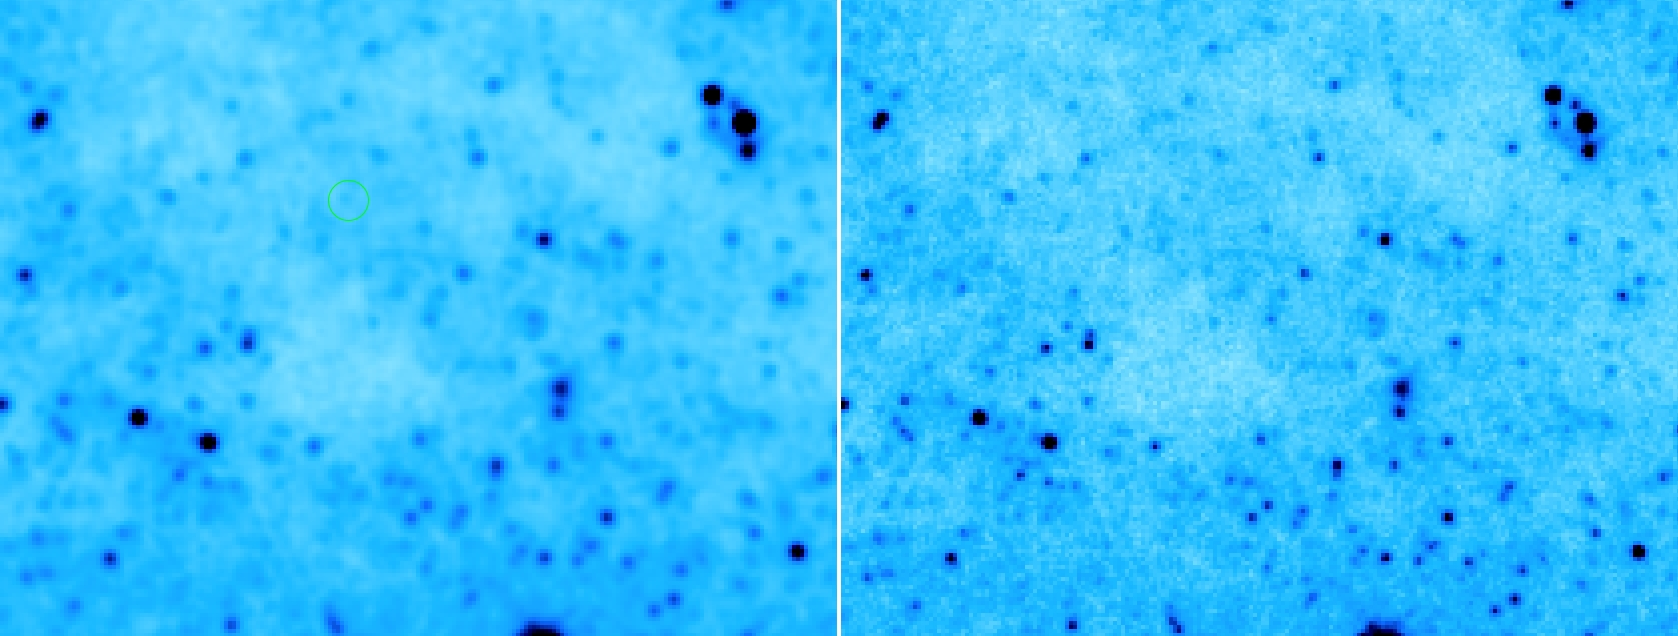
\includegraphics[width=0.87\textwidth]{conv.jpg}
%     \caption{In this image you can observe how an observation looks, before and after convolution, this particular image corresponds to the B band filter and was convolved to a 0.083 arcsec FWHM}
%     \label{img:conv}
% \end{figure}

% \begin{table}[h]
%   \centering
%     \begin{tabular}{ c c c }
%     \hline\hline
    
%     Filter / Config. & Central $\lambda$ & FWHM (arcsec)\\
%     \hline
    
%     F225W & 235.9 nm & $\sim$0.083\\
    
%     F336W & 335.5 nm & $\sim$0.075\\
    
%     F373N & 373.0 nm & $\sim$0.070\\
    
%     F438W & 432.5 nm & $\sim$0.070\\
    
%     F487N & 487.1 nm & $\sim$0.067\\
    
%     F502N & 501.0 nm & $\sim$0.067\\
    
%     F657N & 656.7 nm & $\sim$0.070\\
    
%     F673N & 676.6 nm & $\sim$0.070\\
    
%     F814W & 802.4 nm & $\sim$0.074\\
    
%     \hline
%   \end{tabular}
%   \caption{WFC3/UVIS PSF FWHM informations for the selected dataset, as you can see the largest number here is 0.083 wich means the poorest spatial resolution, this is the number used to calculate the convolution kernel, in order to precess them all images must have the same spatial resolution.}
%   \label{tab:dos}
% \end{table}

% After convoling all the picures, I started to do some tests, but I realized that maybe around 30\% of the images was missing information and/or noise and the results I was getting were mislead by the outliers. In clustering algorithms we must help the algorithm, make sure that what we are inputing is something that can be clustered, although some of them are \emph{shielded} against outliers, making our data more accesible and easy for the neural networks to interpret will help you to get better results, as you can see in image \ref{img:dos} (open one and explore it in DS9) there is missing information and noise. In order to correct this I decided to go with the easiest way I could think of, just cut the image. And I did selected a processable area excluding all the missing information and noisy areas.

% \begin{figure}[h]
% 	\centering
%     \includegraphics[width=0.47\textwidth]{uno.jpg}
%     \caption{Look at the image, it is composed of two mosaics, therefore, there are some regions with missing data, now look at the borders of each mosaic there is noise near the edges, this is data that we don't want messing with our clustering algorithm and can be classifed as outliers, it is very important to reduce them as much as possbile so the output clusters can be correclty classified and correspond to the information that we are looking for}
%     \label{img:dos}
% \end{figure}

% The next step was to build the datacube, at this point you can decide if you want to process your images indendently or all of them. The ideal here is to input all of them in a datacube, so the output cluters relate information from all the wavelenghts and the regions covered by them can be interpreted more easily. Now if you choose to create an imagecube (just append the image arrays in one FITS file) it is posible that youy images have a different conversion between their world coordinate system to pixel, so have to make sure all of your images are projected with only one conversion, this mean that you have to reproject them to a common WCS.

% Well, what I wrote before it is a brief summary of what I did, but I'm sure that you can find a better way to do your own data pre-processing but here are some things that you should consider:
% 	\begin{itemize}
%     	\item Create a methond as general as possible, with input parameter that can be adapted to any kind of data, this will save you a lot of work in the future
%         \item Understand first your algorithm, how the data is going to be processed and design the best way to input your data
%         \item Accomodate your data according to the type of attributes that the algorithm can handle
%         \item Consider the size of your dataset, if it's huge your program may never end
%         \item Find out of your algorithm can work with high dimensional data (multi-wavelenght), because if not, you won't be able to input datacubes
%         \item Find out if your selected clustering algorithms is able to find clusters of irregular shapes, this will help you to device the best way to accomodate your patterns
%         \item Handle outliers, if you identify them, know where they are, try to eliminate them as much as possible, we don't want them messing with our clusters
%         \item In case that you come up with an artful mathematical method like PCA to reduce dimensionality, make sure that what you input can later make sense when is clustered, becuase you will be working in another space
%         \item Remeber that the most important goal is to find hidden knowledge therefore, you must know you to visualize and interpret your results
%         \item For the let's call it \emph{astronomy image processing}, make sure that your data is scientifically aproved ask people around you.
%     \end{itemize}

% %Convolution
% %Cropping
% %Repgojection
% %Cubbing
% %Explain the main rules of why to preprocess the data

% This section is explained at lenght in the GitHub page, there you will find my codes and some helpful links, \url{https://github.com/LaurethTeX/Clustering/blob/master/Preprocessing.md}

% \section{Software available}
% %Como hacer preprocessing en los datos
% For doing data preprocessing there are a bunch of softwares available, even there is one being developed by Sophia Lianou called \emph{imagecube} which, when it is finished, will be one of the best, has everything you need in one package. I'll say that this part is yours to discover, everyday there are more and more being released or new versions of the existent ones but in the meanwhile it will depend entirely on you, which software you want to use. For \emph{Python} all the functions you will need can be found in the \emph{Astropy} module, \textbf{check the API!!!.}


% This specific part is all explained in GitHub in this link. \url{https://github.com/LaurethTeX/Clustering/blob/master/Preprocessing.md#first-step-data-pre-processing}

% \begin{remark}
% 	Some links to start,
%     \begin{itemize}
%     	\item Astropy, Convolution and filtering, \url{http://docs.astropy.org/en/stable/convolution/index.html}
%         \item AstroDrizzle: New Software for Aligning and Combining
% HST Images, With Improved Handling of Astrometric Data, \url{http://drizzlepac.stsci.edu/}
% 		\item Tiny Tim HST PSF Modeling, \url{http://www.stsci.edu/hst/observatory/focus/TinyTim}
%         \item IRAF, Image Reduction and Analysis Facility, \url{http://iraf.noao.edu/}
%     \end{itemize}
% \end{remark}


% %----------------------------------------------------------------------------------------
% %	CHAPTER 4
% %----------------------------------------------------------------------------------------

% \chapterimage{head1.png} % Chapter heading image

% \chapter{Experimenting}

% I discovered surfing on the internet a cloud computing software that is free, has data mining algorithms embeded, is specifically developed for Astronomy and is programmed by Caltech, University Federico II and the Astronomical Observatory of Capodimonte. The homepage website, \url{http://dame.dsf.unina.it/index.html}. Well, the platform for testing is ready!, now what? I requested and account and the next day they sent me an acceptance with my username and my password approved.
% I introduced myself to the documentation, the available clustering funcionts, the manuals for every method, the blogs and discovered that the was one method available that could work with datacubes and do its clustering on every pattern (number in the multidimensional matrix) which was exaclty what I needed. The name of this method is ESOM (Evolving Self Organizing Maps) and I read its manual, did some foolish test with all my image and ... never got a result ... the experiment ran forever (more than two weeks), when I realised that this wasn't the best way to tackle this problem I started considering only clustering on the independent images and not in the datacube due to the fact that the dimensionality was inmense. So, in the end my selected methods have some results but not all, here is where all the work has to be done, analyzed and tested again.

% \section{Methods Selected}

% \subsection{ESOM, Evolving Self Organizing Maps}
% The \emph{official} manual for this method can de found here, \url{http://dame.dsf.unina.it/documents/ESOM_UserManual_DAME-MAN-NA-0021-Rel1.2.pdf}, there you will find a full explanation of the method, the meaning of every variable and the supported file types.

% Here is my own explanation of how this particular method works, first of all, can be used as an unsupervised machine learning technique or you can help the algorithm to identify regions an make it a supervised machine learnig technique, this type of clustering finds groups of patterns with similarities and preserves its topology, starts with a null network without any nodes and those are creted incrementally when a new input pattern is presented, the prototype nodes in the network compete with each other and the connections of the winner node are updated. 

% The method is divided in three stages, \emph{Train}, \emph{Test} and \emph{Run}.
% The first step to experiment with this method is Train. Here, the important variables to undertand an look at are, the learning rate, epsilon and the pruning frequency. It is highly recomendable that you check the DAMEWARE manual for this function, there they will explain in detail the meaning of each on the mentioned variables.
% % fULL AND SAMPLE DATACUBE
% \subsubsection{Expected Results}
% 	This particular method as I mentioned before supports datacubes and considers as an independent pattern all the  numbers in the multi-dimensional array this means that our clusters are groups of patterns with similar characteristics, that correspond to volumes of similar fluxes of electrons inside the datacube.
    
%     The output files from the experiment that will show us our results are, 
%     \begin{itemize}
%     	\item \emph{E\_SOM\_Train\/Test\/Run\_Results.txt}: File that, for each pattern, 
% reports ID, features, BMU, cluster and activation of winner node
% 		\item \emph{E\_SOM\_Train\/Test\/Run\_Histogram.png}: Histogram of clusters found 
%         \item \emph{E\_SOM\_Train\/Test\/Run\_U\_matrix.png}: U-Matrix image 
%         \item \emph{E\_SOM\_Train\/Test\/Run\_Clusters.txt}: File that, for each clusters, reports label, number of pattern assigned, percentage of association respect total number of pattern and its centroids. 
%         \item \emph{E\_SOM\_Train\_Datacube\_image.zip}: Archive that includes the 
% clustered images of each slice of a datacube.\footnote{I have my doubts whether this file is produced or not, in none of my test was produced, you might need to contact the developers and ask about this.}
%     \end{itemize}
% The file that you will be looking forward to see is the last one, the zip where you will be able to see the slices of the volume, and how the final configuration of the clusters was arranged.

% \subsubsection{Failed and still running tests: What no to do and what is still running}
% The first tests I did included all the complete datacube, including the areas where data was missing, the images were only reprojected and convolved. That was before realising that outliers migth affect the ability of the algorithm to identify the clusters and distract them with noise and missing data. So, the first thing you must NOT do, is to get rid of the outliers when you are training your network, if you ever get to have a well trained network then it might be interesting to learn how the network interacts with noise an outliers, but for now we will help her a bit. 

% In table \ref{tab:ds9failed} are the input parameters I used to the failed tests applied in the \emph{raw} datacube, and in table \ref{tab:ds9running} are the input parameters used on experimets that are stil running since August 7th, 2014. (I wonder if they will ever end)

% \begin{table}[h!]
%   \centering
%     \begin{tabular}{ c c c c c c }
%     \hline\hline
    
%     Name & Input nodes & Normalized data & Learning rate & Epsilon & Pruning Frequency\\
%     \hline
    
%     Train2 & 1 & 1 & 0.3 & 0.001 & 5\\
%     Train3 & 1 & 1 & 0.7 & 10 & 100\\
%     Train4 & 1 & 1 & 0.95 & 1 & 10\\
%     Train5 & 1 & 1 & 0.99 & 0.1 & 10\\
%     Train6 & 1 & 1 & 0.01 & 0.01 & 1\\
%     Train7 & 1 & 1 & 0.5 & 0.7 & 5\\
%     Train8 & 1 & 1 & 0.5 & 0.5 & 7\\
%     Train11 & 1 & 1 & 0.25 & 0.00001 & 10\\
    
%     \hline
%   \end{tabular}
%   \caption{This table describes all the failed experiments done in the workspace WFC3 with the \emph{raw} datacube as an input, using the ESOM method in the DAME platform selecting the number 3 as the dataset type and without using a previous configuration file.}
%   \label{tab:ds9failed}
% \end{table}

% \begin{table}[h!]
%   \centering
%     \begin{tabular}{ c c c c c c }
%     \hline\hline
    
%     Name & Input nodes & Normalized data & Learning rate & Epsilon & Pruning Frequency\\
%     \hline
    
%     Train9 & 1 & 1 & 0.3 & 0.0001 & 5\\
%     Train10 & 1 & 1 & 0.99 & 0.0001 & 10\\
%     Train12 & 1 & 1 & 0.5 & 0.0001 & 5\\
    
%     \hline
%   \end{tabular}
%   \caption{This table describes all the experiments done in the workspace WFC3 that are still running since August 7th, 2014 with the \emph{raw} datacube as an input, using the ESOM method in the DAME platform selecting the number 3 as the dataset type and without using a previous configuration file.}
%   \label{tab:ds9running}
% \end{table}

% Some of the failed experiments had histogram like the one you can see on figure \ref{img:faildtrain2} where the cluters were created but reached a point where the neural network could not define how to differenciate a cluster from another clusted and failed.

% \begin{figure}[h!]
% 	\centering
%     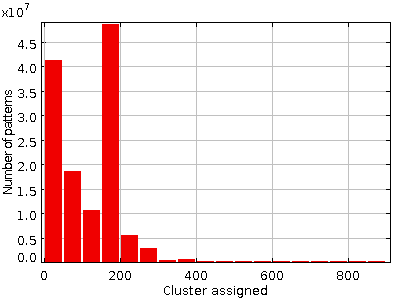
\includegraphics[width=0.47\textwidth]{Histogram_train2.png}
%     \caption{In this particular experiment, the neural network failed due to a very low prunning frequency, high number of patterns and all the outliers inclusions.}
%     \label{img:faildtrain2}
% \end{figure}

% Hey, if you were wondering why I always choose to normilize, and one as the input node, well the normalization is due to the fact that I know that the data has, according to its filter, all kinds of ranges of fluxes on every layer which means that the distances between patterns might not be correct, this is a topic you should look into. And for the input node I choose 1 because if I start with any other number the experiment automatically fails, and of course we do not want that.

% As I progressed and saw the results and the \emph{log files} in all the failed experiments I decide to try the algorithm on independent layers and see if I could get something. Therefore I selected the H$\alpha$ convolved observation (halpha\_conv.fits) and did some tests on it, table \ref{tab:hafailed} shows the parameters I used for the failed experiments and table \ref{tab:harun} shows the paramters fo the still running experiments.

% \begin{table}[h!]
%   \centering
%     \begin{tabular}{ c c c c c c }
%     \hline\hline
    
%     Name & Input nodes & Normalized data & Learning rate & Epsilon & Pruning Frequency\\
%     \hline
    
%     TrainHa1 & 1 & 1 & 0.5 & 0.01 & 5\\
%     TrainHa2 & 1 & 1 & 0.5 & 0.001 & 5\\
    
%     \hline
%   \end{tabular}
%   \caption{This table describes the failed experiments done in the workspace WFC3 for the \emph{halpha\_conv.fits} file, using the ESOM method for one layer in the DAME platform selecting the number 3 as the dataset type and without using a previous configuration file.}
%   \label{tab:hafailed}
% \end{table}

% \begin{table}[h!]
%   \centering
%     \begin{tabular}{ c c c c c c }
%     \hline\hline
    
%     Name & Input nodes & Normalized data & Learning rate & Epsilon & Pruning Frequency\\
%     \hline
    
%     TrainHa3 & 1 & 1 & 0.5 & 0.0001 & 5\\
    
%     \hline
%   \end{tabular}
%   \caption{This table describes the still running experiments since August 10th, 2014 in the workspace WFC3 for the \emph{halpha\_conv.fits} file, using the ESOM method for one layer in the DAME platform selecting the number 3 as the dataset type and without using a previous configuration file.}
%   \label{tab:harun}
% \end{table}

% My next mental step was to repeat the tests eliminating as many outliers I could reduce, my hypothesis here is that, if I elimante all the areas where there is missing data and noise, the neural networks will be concentrated only in the patterns I'm interested in clustering and maybe idenfying interesting regions that correspond to some known interstellar object. So, what I did was to try the ESOM algorithm with, again, independent images, this time I decided to apply the same experiment to three different layers, H$\alpha$, UV wide and $i$-band. In table \ref{tab:threefail} you can see the parameters of the failed experiments and on figure \ref{img:fail3} there are some of the output histograms. Also, in table \ref{tab:threerun} you can see the input parameters of the still running experiments.

% \begin{table}[h!]
%   \centering
%     \begin{tabular}{ c c c c c c }
%     \hline\hline
    
%     Name & Input nodes & Normalized data & Learning rate & Epsilon & Pruning Frequency\\
%     \hline
    
%     Train1 & 1 & 1 & 0.5 & 0.001 & 50\\
%     Train2 & 1 & 1 & 0.5 & 0.01 & 50\\
%     Train3 & 1 & 1 & 0.5 & 0.1 & 100\\
%     Train4 & 1 & 1 & 0.5 & 0.001 & 100\\
    
%     \hline
%   \end{tabular}
%   \caption{This parametes where used in three different workspaces (\emph{halphaCrop, uvwidecrop, ibandcrop}), with their own input file that corresponded to the convolved and cropped observation of each filter (halpha\_conv\_crp.fits, uvwide\_conv\_crp.fits, iband\_conv\_crp.fits), all of the experiments had no previous configuration file and the dataset type was 3 and all failed.}
%   \label{tab:threefail}
% \end{table}

% \begin{figure}[h!]
% 	\centering
%     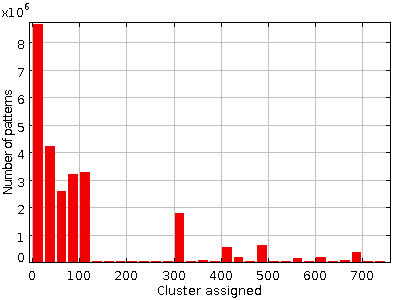
\includegraphics[width=0.31\textwidth]{Histogram-halpha1.png}
%     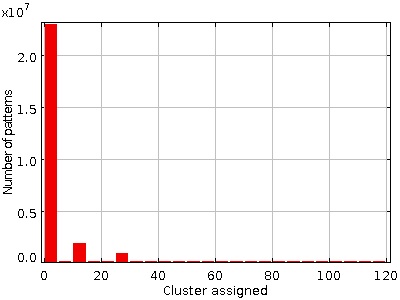
\includegraphics[width=0.31\textwidth]{Histogram-uvwide-2.png}
%     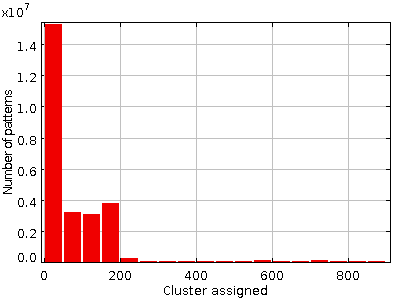
\includegraphics[width=0.31\textwidth]{Histogram-iband3.png}
%     \caption{The histogram on the left corresponds to the halpha workspace in Train1, the one on the center to the iband workspace in Train3 and the one on the right to the uvwide workspace in Train2, all of them were failed experiments.}
%     \label{img:fail3}
% \end{figure}

% \begin{table}[h!]
%   \centering
%     \begin{tabular}{ c c c c c c }
%     \hline\hline
    
%     Name & Input nodes & Normalized data & Learning rate & Epsilon & Pruning Frequency\\
%     \hline
    
%     Train5 & 1 & 1 & 0.5 & 0.0001 & 100\\
%     Train6 & 1 & 1 & 0.99 & 0.0001 & 75\\

%     \hline
%   \end{tabular}
%   \caption{This parametes where used in three different workspaces (\emph{halphaCrop, uvwidecrop, ibandcrop}), with their own input file that corresponded to the convolved and cropped observation of each filter (halpha\_conv\_crp.fits, uvwide\_conv\_crp.fits, iband\_conv\_crp.fits), all of the experiments had no previous configuration file and the dataset type was 3. The experiments mentioned are still running since August 11th, 2014.}
%   \label{tab:threerun}
% \end{table}

% As you can see, I discovered that if I choose an epsilon of 0.0001 the experiments will be still running, and all of the other variables can be variated like the learning rate and the pruning frequency.

% \subsubsection{The big and small reprojected datacube}
% After a few days of waiting anxiously for the experiments to end and not getting any new results I decided to test the convolved, cropped and reprojected datacube including all the layers with a fixated prunning frequency of 0.0001, hopping that this time I could get some interesting results. The input parameters for the two experiments I tested can be seen in table \ref{tab:cubeesom}.

% \begin{table}[h!]
%   \centering
%     \begin{tabular}{ c c c c c c }
%     \hline\hline
    
%     Name & Input nodes & Normalized data & Learning rate & Epsilon & Pruning Frequency\\
%     \hline
    
%     ESOMtrain1 & 1 & 1 & 0.5/0.75 & 0.0001 & 100\\
%     ESOMtrain2 & 9 & 1 & 0.75 & 0.001 & 100\\

%     \hline
%   \end{tabular}
%   \caption{This parametes where used in two different workspaces (\emph{DataCube, RPDataCube}), the first experiment is still running since August 12th, 2014 and the second failed. The input for the DataCube workspace corresponds to a 9 layer datacube with no reprojection and the RPDataCube input is the same datacube but reprojected.}
%   \label{tab:cubeesom}
% \end{table}

% As you can see, in the experiment \emph{ESOMtrain2} I tried to start the neural network with 9 nodes (thinking logically as having 9 layers in the datacube) and immediatly the experiment failed, so \textbf{do not try to input a number different than one.}

% I waited 17 days for the experiments to finish (I did some other stuff in the meanwhile, most of the time learning new things) but I did not get any results so I came up with a different strategy, selecting small datacubes with already identified regions by the NED database. I selected randomly a particular HII region located in RA 204.26971, DEC -29.84933 (See figure \ref{img:h2region}) and centered it in a 605x605 pixels sample.

% \begin{figure}[h!]
% 	\centering
%     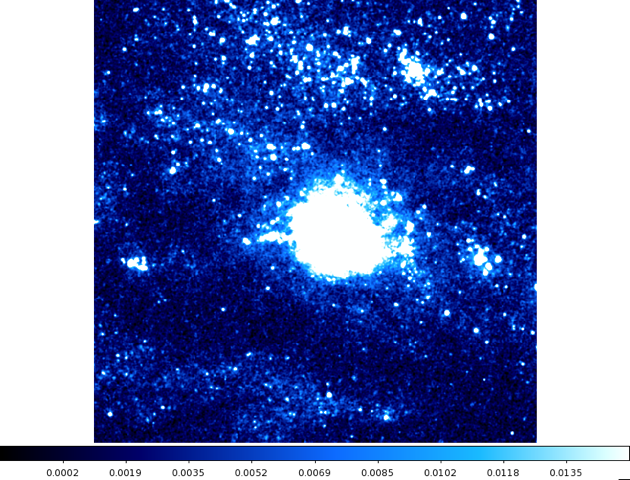
\includegraphics[width=0.52\textwidth]{small_ex.png}
%     \caption{Illustration of the randomly chosen HII region for the small sample from the M83 reprojected datacube.}
%     \label{img:h2region}
% \end{figure}

% This time, most of the experiments gave me immediate results failing or finishing. On table \ref{tab:small}, you can see the input parameters and the status of the experiments I tested with the small datacube.

% \begin{table}[h!]
%   \centering
%     \begin{tabular}{ c c c c c c }
%     \hline\hline
    
%     Name & Normalized & Learning rate & Epsilon & Pruning Frequency & Status\\
%     \hline
    
%     ESOMtrain1 & 0 & 0.5 & 0.001 & 50 & Running\\
%     Train2 & 1 & 0.5 & 0.0001 & 50 & Ended\\
%     Train3 & 1 & 0.5 & 0.1 & 50 & Ended\\
%     Train4 & 0 & 0.5 & 0.0001 & 50 & Running\\
%     Train5 & 0 & 0.95 & 0.0001 & 100 & Running\\
%     Train6 & 1 & 0.99 & 0.001 & 50 & Ended\\

%     \hline
%   \end{tabular}
%   \caption{All the mentioned experimend belong to the SmallDataCube workspace, have 3 as data type and one input node, no previous configuration file and the input file is \emph{rp\_small\_datacube.fits}.}
%   \label{tab:small}
% \end{table}
% In this case three of the experiments ended and none od them failed (yet), here I detected that the output file that contains the distributions of the clusters on every layer is missing, but we got some interesting resuts, in the next figures (\ref{img:smallended},\ref{img:matrixended}) you can apreciate better what I'm taking about.

% \begin{figure}[h!]
% 	\centering
%     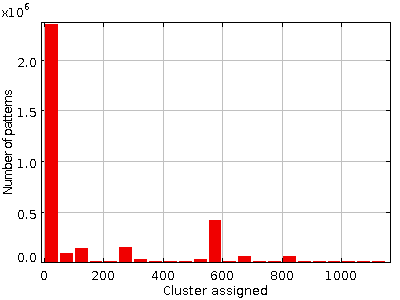
\includegraphics[width=0.31\textwidth]{Small-train2.png}
%     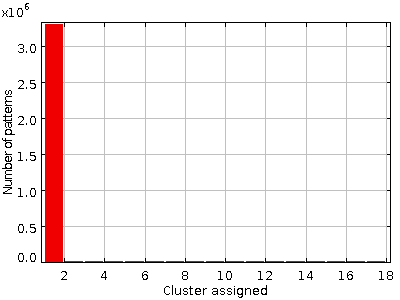
\includegraphics[width=0.31\textwidth]{Small-train3.png}
%     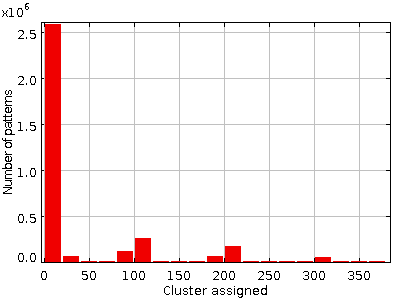
\includegraphics[width=0.31\textwidth]{Small-train6.png}
%     \caption{All of the images correspond to histograms of the ended experiments mentioned above in order (Train2, Train3, Train6), as you can see there is a predominance on one of the clusters that can mean that is detecting the HII region or the experiment never started, to understand further the results a visualization of the clusters is needed.}
%     \label{img:smallended}
% \end{figure}

% \begin{figure}[h!]
% 	\centering
%     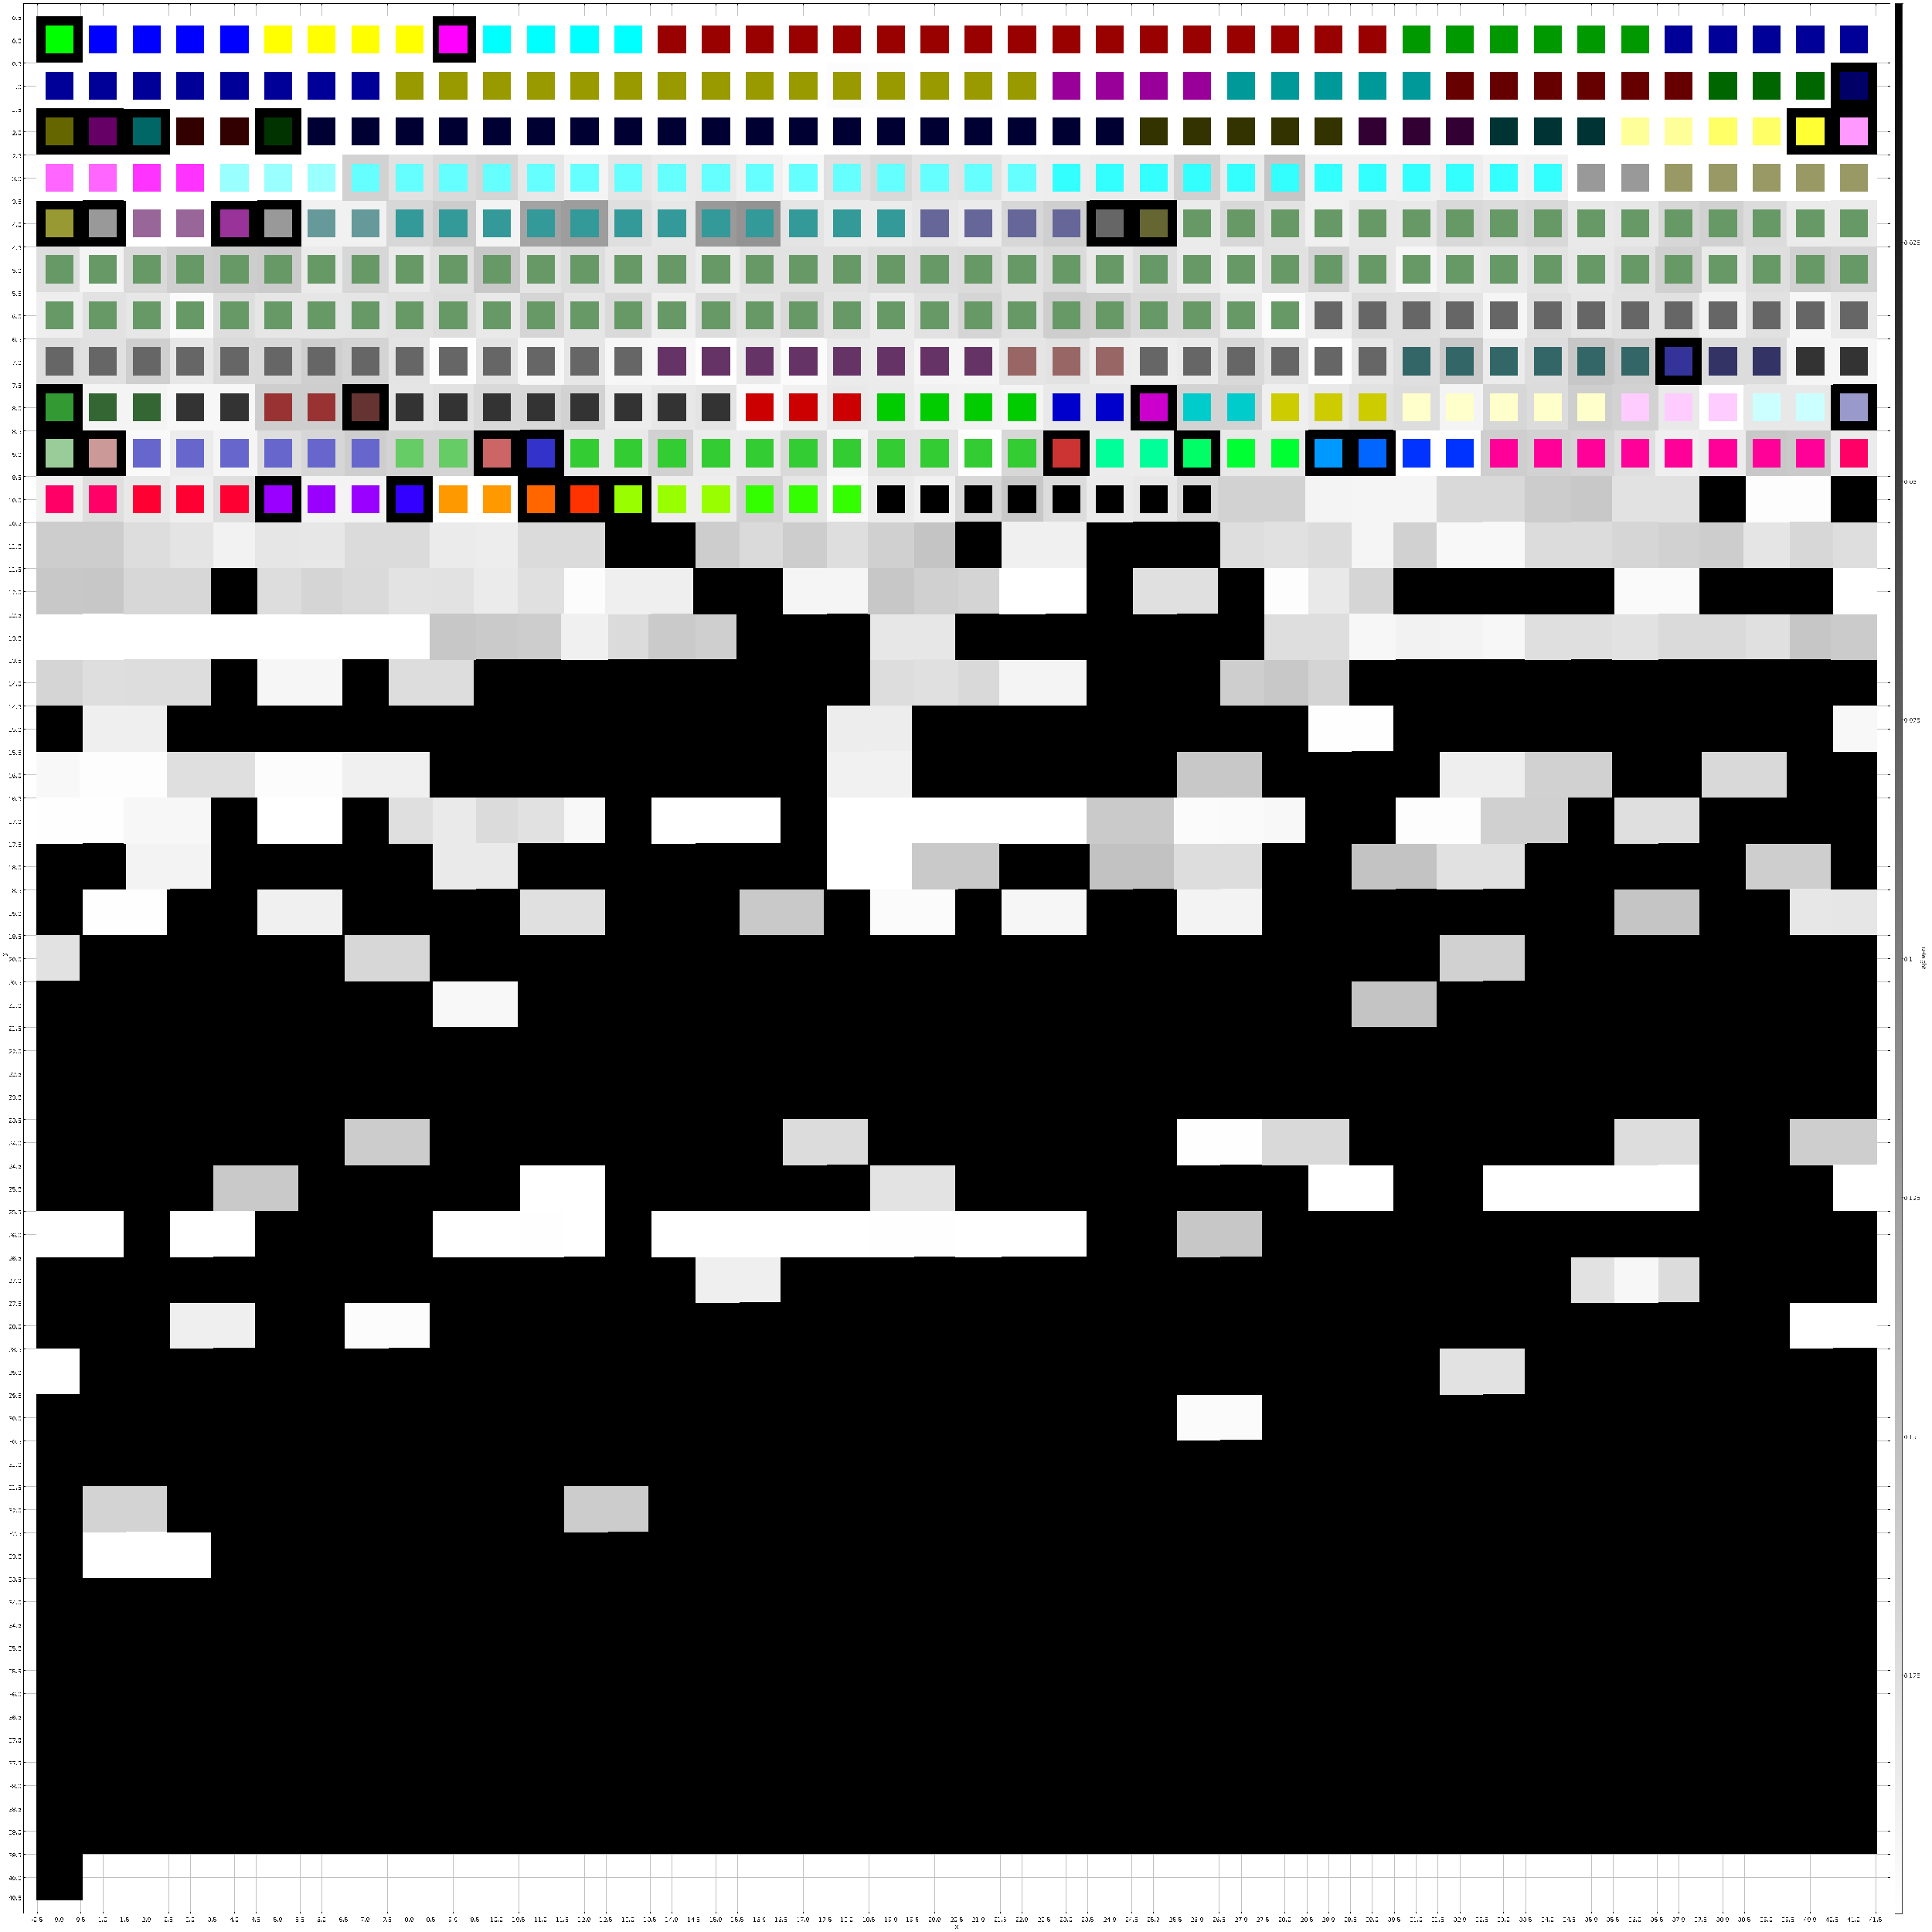
\includegraphics[width=0.31\textwidth]{matrix2-01.png}
%     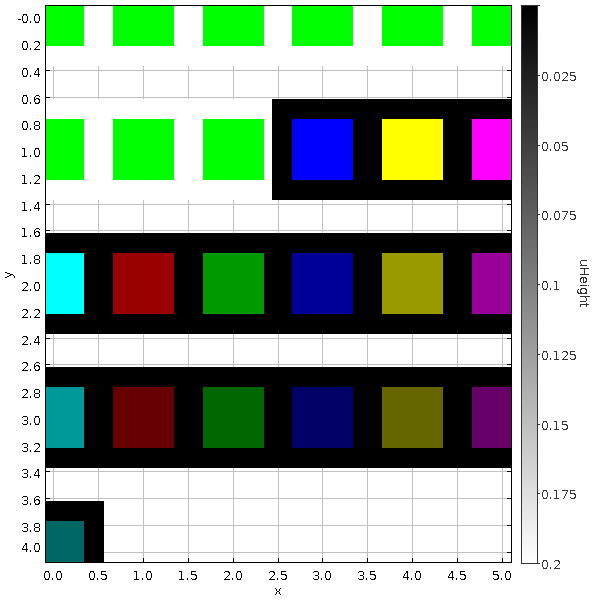
\includegraphics[width=0.31\textwidth]{Small-train3-matrix.png}
%     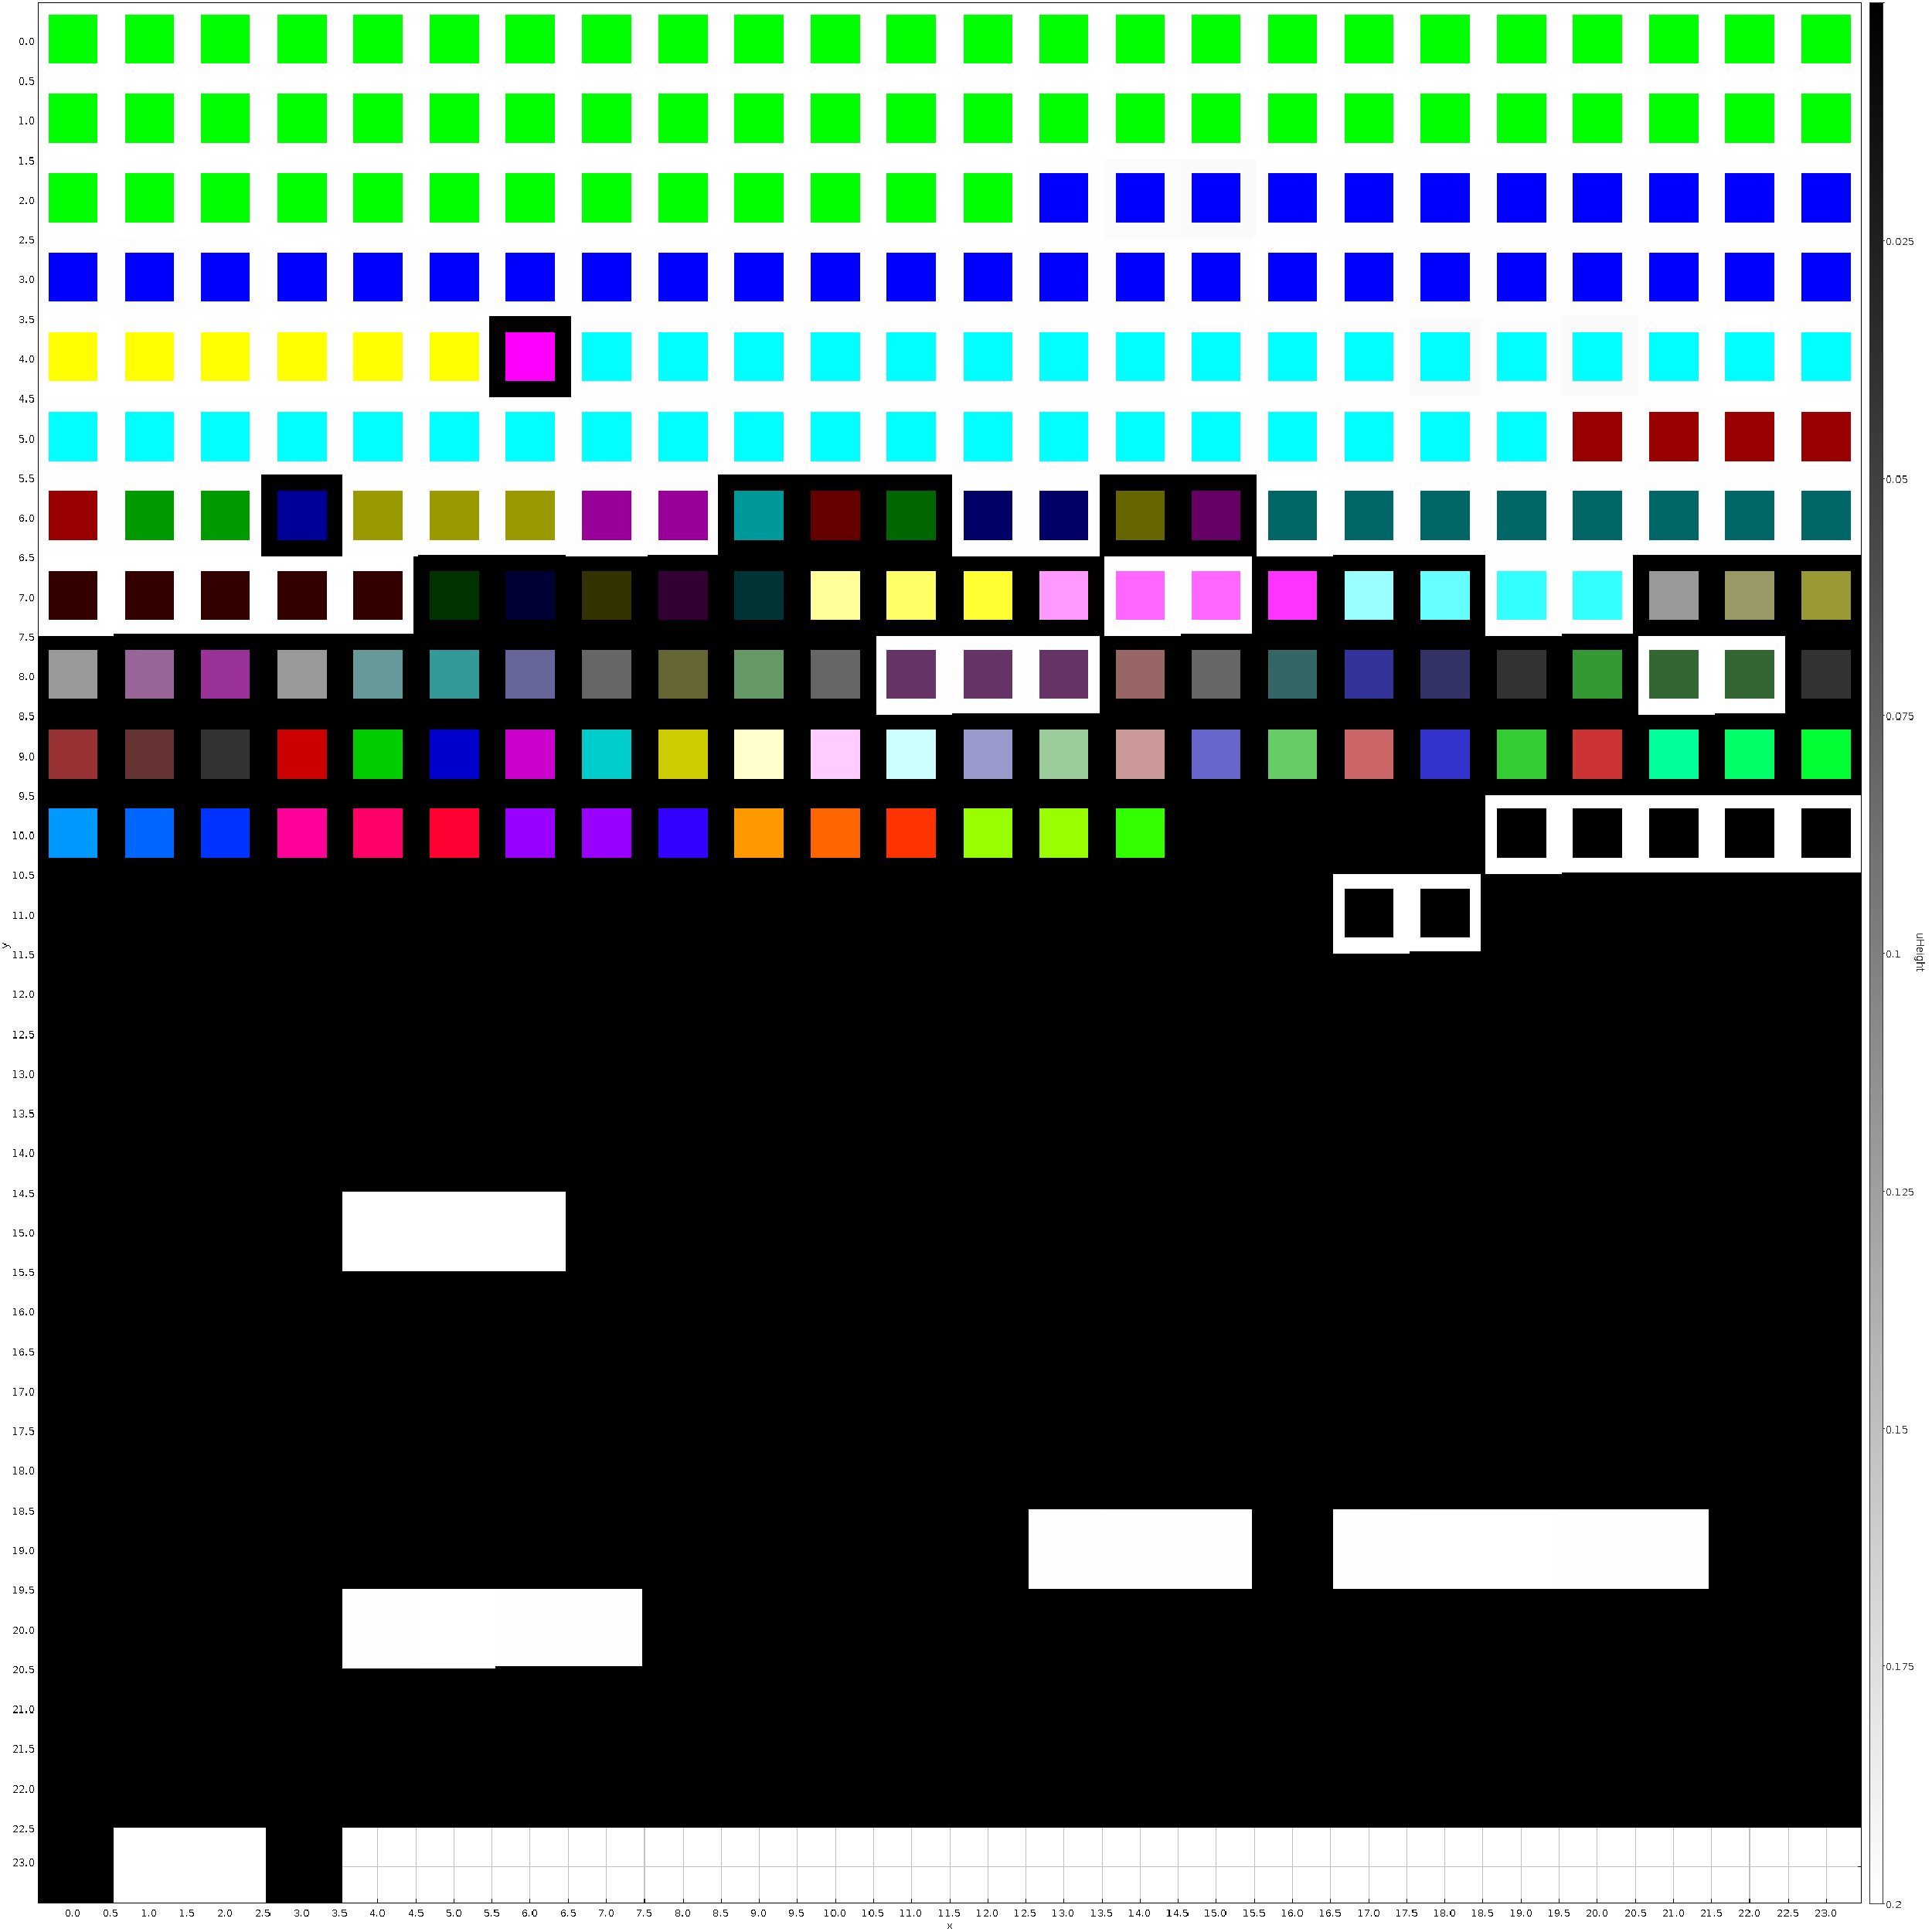
\includegraphics[width=0.31\textwidth]{matri6-01.png}
%     \caption{All of the images correspond to U-matrices of the ended experiments mentioned above in order (Train2, Train3, Train6)}
%     \label{img:matrixended}
% \end{figure}
%  There is work to be done for this cases, understand what is going on and interpret correctly the results, but last we got some.
% \subsection{CSOM}
% %one image
% Well, as I mentioned before I did some tests using the ESOM method but since I wasn{t getting any results I thougth of testing this methond, as always I strongly recommend to read carefully its manual, \url{http://dame.dsf.unina.it/documents/SOFM_UserManual_DAME-MAN-NA-0014-Rel1.1.pdf} and fully undesrtand what is going on behind the curtains. In the meanwhile, this is my own explanation. This method uses FITS files, does not support datacubes, speciffically uses a neighborhood function in order to preserve the topological properties of the input space, it is a type of artificial network and is mainly unsupervised learning  and produces a low dimensional discretized representation of the input space of the training samples. I in this case you can choose the number of clusters/neurons in the first layer (neural network), the diameter, number of layers (in the neural network), learning rate and variance  on each layer. Here you have more input parameters to control.
% \subsubsection{Expected Results}
% Well in this case, since only FITS images are allowed, what we expect to find are areas indeitfying the different objects in the interstellar medium.

% The important results in this case, are got in the \emph{Run} and \emph{Test} steps, in the \emph{Train} step only the network configuration is outputted. What we are interested on seein are the plotted clusters.
% \subsubsection{Tests}
% In this case I did some tests on the CSOM workspace, but none of the, where succesful, too many input variables to control and test. So, in this case I will leave this parameters free for you to try. I do believe that tis method could be very useful and if you find a way to input the datacube in a different configuration you will get some interesting results, due to the fact that in this method the preservation of the topology is one of the main principles.
% %Mencionar los dos metodos de DAMEWARE
% %Explicar los dos metodos, como untroduciste los datos, el objectivo de cada uno

% %Lo que se espera obtener de cada uno de los experimentos, uno es en una sola imagen y el otro es en el datacube
% %Los archivos que se obtienen y lo que significas, lo que se puede hacer



% %Poner los parametros que se han elegido en los experimentos fallidos, y los que siguen en modo running
% %Exlpicar por fases los experimentos que se intentaron


% \section{Further work}
% Well, finally we reached the point where I my time in Canada finished and I this research is still on its first stages. I have so many ideas of how to explore the clustering techniques in the DAME platform, MatLab, Python and everything else that can be tested. 

% \subsection{Some interesting ideas}
% %Normalizar los datos
% %Acomodarlos y hacer que los paquetes sean mas pequeños
% %Random points
% For now, I would say that your best chance here, is to device an efficient way to input the information contained in a datacube as a list of points with values and reduce its dimensionality by randomly choosing them on every layer. If you are ever stuck, or no new ideas come to your mind, do not hesitate to contact me I might have a new interesting idea you can test.

% \subsection{Links you should check out}
% Most of them are listed in the useful resourses section of The Caltech-JPL Summer School on Big Data Analytics, the webpage \url{https://class.coursera.org/bigdataschool-001/wiki/Useful_resources}, you may need to create an account in Coursera and enroll in the course. And the rest of them are located in the References section on my GitHub page, \url{https://github.com/LaurethTeX/Clustering/blob/master/References.md}.
% %Los links que estan en la pagina de el curso de caltech
% %Sky surveys
% %MATLAB SOM toolbox
% %SAO datamining
\vfill
% \textit{Wish you all the best, Andrea Hidalgo}
\end{document}